%%
%% This is file `squelette-rr.tex',
%% generated with the docstrip utility.
%%
%% The original source files were:
%%
%% RR.dtx  (with options: `sample')
%% ********************************************************************
%% Copyright (C) 1997-1999 2004 2006-2011 INRIA/APICS/MARELLE by Jose' Grimm
%% This file may be distributed and/or modified under the
%% conditions of the LaTeX Project Public License, either version 1.3
%% of this license or (at your option) any later version.
%% The latest version of this license is in
%%    http://www.latex-project.org/lppl.txt
%% and version 1.3 or later is part of all distributions of LaTeX
%% version 2003/12/01 or later.
%% An archive of the software can be found at
%%    ftp://ftp-sop.inria.fr/marelle/RR-INRIA

\documentclass[twoside]{article}
\usepackage[a4paper]{geometry}
\usepackage[utf8]{inputenc} % ou \usepackage[utf8]{inputenc}
\usepackage[T1]{fontenc} % ou \usepackage[OT1]{fontenc}
\usepackage{RR}
\usepackage{hyperref}
%\usepackage{subfigure}
\usepackage{subfig}
\usepackage{caption}
\usepackage{cite}
\usepackage{todonotes}
\usepackage{filecontents}
\usepackage{listings}
%%\usepackage[frenchb]{babel} % optionnel
\RRNo{7003}
%% \RTNo{0703}
%%
%% date de publication du rapport
\RRdate{April 2015}
%%
%% Cas d'une version deux
%% \RRversion{2}
%% date de publication de la version 2
%% \RRdater{November 2008}
%%
\RRauthor{% les auteurs
 % Premier auteur, avec une note
H\'el\'ene Coullon\thanks{Footnote for first author}%
  % note partag\'ee (optionnelle)
  \thanks[sfn]{Shared foot note}%
 % \and entre chaque auteur s'il y en a plusieurs
  \and
Christian Perez\thanks{Footnote for second author}%
 % r\'ef\'erence \`a la note partag\'ee
%\thanksref{sfn}
 % liste longue pour tests de mise en page
%\and Nicolas Bourbaki\thanks{etc} \and Andr\'e Lichnerowicz
%\and Marcel-Paul Sch\"utzenberger \and Jacques-Louis Lions
}
%% Ceci apparait sur chaque page paire.
\authorhead{Coullon \& Perez}
%% titre francais long
\RRtitle{Exemple de document\\
 utilisant le style\\rapport de recherche\\Inria}
%% English title
\RRetitle{A Component-Based and Parallel Multi-Stencil DSL}
%%
%\titlehead{Example of RR.sty}
%%
%\RRnote{This is a note}
%\RRnote{This is a second note}
%%
\RRresume{Resume en francais
}
\RRabstract{
abstract }
%%
\RRmotcle{mots-cles}
%%
%% \RRprojet{Apics}  % cas d'un seul projet
\RRprojets{Avalon}
%%
%% \URLorraine % pour ceux qui sont \`a l'est
%% \URRennes  % pour ceux qui sont \`a l'ouest
%\URRhoneAlpes % pour ceux qui sont dans les montagnes
%% \URRocq % pour ceux qui sont au centre de la France
%% \URFuturs % pour ceux qui sont dans le virtuel
%% \URSophia % pour ceux qui sont au Sud.
%%
%% \RCBordeaux % centre de recherche Bordeaux - Sud Ouest
%% \RCLille % centre de recherche Lille Nord Europe
%% \RCParis % Paris Rocquencourt
%% \RCSaclay % Saclay \^Ile de France
 \RCGrenoble % Grenoble - Rh\^one-Alpes
%% \RCNancy % Nancy - Grand Est
%% \RCRennes % Rennes - Bretagne Atlantique
%\RCSophia % Sophia Antipolis M\'editerran\'ee
%\newtheorem{mydef}{\textbf{Definition}}
%\newtheorem{myprop}{\textbf{Property}}

\usepackage{amsmath}
\usepackage{amssymb}

\newtheorem{theorem}{Theorem}[section]
\newtheorem{myprop}[theorem]{Proposition}
%\newtheorem{corollary}[theorem]{Corollary}

\newenvironment{proof}[1][Proof]{\begin{trivlist}
\item[\hskip \labelsep {\bfseries #1}]}{\end{trivlist}}
\newenvironment{mydef}[1][Definition]{\begin{trivlist}
\item[\hskip \labelsep {\bfseries #1}]}{\end{trivlist}}
\newenvironment{myth}[1][Theorem]{\begin{trivlist}
\item[\hskip \labelsep {\bfseries #1}]}{\end{trivlist}}
%\newenvironment{example}[1][Example]{\begin{trivlist}
%\item[\hskip \labelsep {\bfseries #1}]}{\end{trivlist}}
%\newenvironment{remark}[1][Remark]{\begin{trivlist}
%\item[\hskip \labelsep {\bfseries #1}]}{\end{trivlist}}

\def\pprec{\mathrel{\scalebox{.9}[1]{$\prec$}\mkern-3mu%
  \scalebox{.4}[1]{$\prec$}\mkern-5.5mu\scalebox{.4}[1]{$\prec$}}}

\newcommand{\qed}{\nobreak \ifvmode \relax \else
      \ifdim\lastskip<1.5em \hskip-\lastskip
      \hskip1.5em plus0em minus0.5em \fi \nobreak
      \vrule height0.75em width0.5em depth0.25em\fi}

\usepackage{graphics}
\usepackage{tikz}
\usepackage[ruled,noend]{algorithm2e}
\usetikzlibrary{calc,arrows,shapes,automata,petri,positioning,decorations.markings,shadows}

\newcommand{\rmq}[1]{\todo[inline,color=red!80]{#1}}

\tikzset{
    use/.style={
    circle,draw=black,fill=black,scale=0.5,text=white
    },
    provide/.style={
    circle,draw=black,fill=white,scale=0.5
    },
    component/.style={
    rectangle,rounded corners=3pt,draw=black
    },
    dcomponent/.style={
    rectangle,rounded corners=3pt,dashed,draw=black
    },
    smallcp/.style={
    rectangle,rounded corners=3pt,draw=black,font=\tiny,
    },
    resource/.style={
    rectangle,rounded corners=3pt, dashed,draw=black,font=\tiny,
    },
    connection/.style={
    decoration={ markings,
      mark=at position 1 with {\node[fill=black,draw=black,circle,inner sep=2pt](conn){};}
      },
    postaction={decorate}
    },
    bconnection/.style={
    decoration={ markings,
      mark=at position 1 with {\node[fill=black,draw=black,circle,inner sep=2pt](conn){};}
      },
    postaction={decorate}
    },
    mpiconn/.style={
    decoration={ markings,
      mark=at position 0.99 with {\node[fill=black,draw=black,rectangle,,inner sep=2pt](mpi){};}
      },
    postaction={decorate}
    },
}


%%
\begin{document}

%%
%\makeRR   % cas d'un rapport de recherche
%% \makeRT % cas d'un rapport technique.
%% a partir d'ici, chacun fait comme il le souhaite

\tableofcontents

%------------------------------------------------------------------------------
% \section{Introduction}
% \label{sect:introduction}
%------------------------------------------------------------------------------
\section{Computational model of Multi-Stencil Programs}
\label{sect:formalism}
To numerically solve a set of PDEs, iterative methods (finite difference, finite volume or finite element methods) are frequently used to approximate the solution through a discretized (step by step) phenomena. Thus, the continuous time and space domains are discretized so that a set of numerical computations are iteratively (time discretization) applied onto a mesh (space discretization). In other words, the PDEs are transformed to a set of numerical computations applied at each time step on elements of the discretized space domain. Among those numerical computations are found a set of numerical schemes, also called \textit{stencil computations}, a set of auxiliary computations also called \emph{local computations}, and finally a set of \emph{reductions} to reduce a bunch of values to a single scalar value.
This section gives formal definitions of what we call a \textit{stencil program} and its computations. Then, the different mid-grain parallelization techniques which can be applied on such program, are presented.

We denote stencil kernels discretized explicit numerical schemes which involve neighborhood computations, whatever the type of space discrtization is (mesh).

%-------------------------------------
\subsection{Time, mesh and data}

$\Omega=\mathbb{R}^n$ is the continuous space domain of a numerical simulation. %For example, if $n=3$, any geographic point on earth could be represented in this space in a given geographic coordinate system.
A mesh $\mathcal{M}$ defines the discretization of the continuous space domain $\Omega$ of a set of PDEs and is defined as follows.

\begin{mydef}
A mesh is a connected undirected graph $\mathcal{M}=(V,E)$, where $V\subset \Omega$ is the set of vertices and $E\subseteq V^2$ the set of edges. The set of edges $E$ of a mesh $\mathcal{M}=(V,E)$ does not contain bridges. It is said that the mesh is applied onto $\Omega$.
\end{mydef}
\begin{figure}[!h]\begin{center}
  \resizebox{8cm}{!}{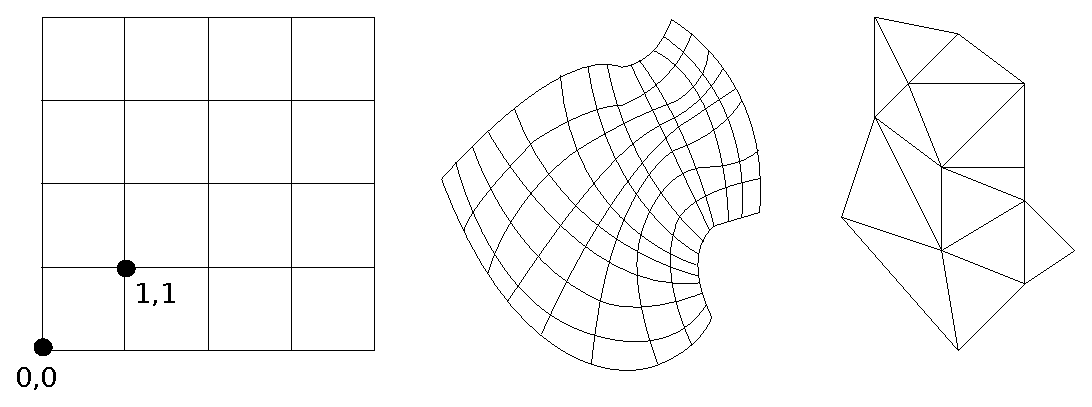
\includegraphics{./images/maillages.pdf}}
  \caption{From left to right, Cartesian, curvilinear and unstructured meshes.}
  \label{fig:mesh}
\end{center}\end{figure}
\begin{mydef}
The dimension of a mesh $\mathcal{M}=(V,E)$ applied onto $\Omega=\mathbb{R}^n$ is denoted $dim(\mathcal{M})=n$.
\end{mydef}
A mesh can be structured (as Cartesian or curvilinear meshes), unstructured, regular or irregular (without the same topology for each element) and hybrid as illustrated in Figure~\ref{fig:mesh}.

\medskip
\noindent \textbf{Definitions}
%\begin{mydef}
\begin{itemize}
\item An entity $e$ of a mesh $\mathcal{M}=(V,E)$ is defined as a subset of its vertices and edges, $e\subset V\cup E$.
\item A group of mesh entities is denoted $E$ such that $E \in \mathcal{P}(V\cup E)$. It represents a set of entities of the same type.
\item The set of mesh entities groups of a simulation is denoted $\mathcal{E}$.
\item Finally, the mesh on which is applied a group of mesh entities $E$ is denoted $mesh(E)$
\end{itemize}
%\end{mydef}

For example, in a 2D Cartesian mesh an entity could be a cell, made of four vertices and four edges, or simply a vertex. As a result, a group of cells and a group of vertices could be defined in $\mathcal{E}$. %This type can be defined as the sets containing exactly four vertices and four edges connected as a cycle. Another type of entities simply are the vertices ($V$) and can be defined as all singletons formed of a single vertex of $V$.

\medskip
This covers the space discretization, however there is also the time dimension which has to be discretized in the simulation.

\medskip
\noindent \textbf{Definitions}
%\begin{mydef}
\begin{itemize}
\item We denote a scalar as an identifier associated to a numerical value and applied onto a mesh $\mathcal{M}$ where $dim(\mathcal{M})=0$. In other words a scalar can be seen as a variable containing a numerical value. The set of scalars is denoted $\mathcal{S}$.
\item $\mathcal{T}=\mathbb{R}$ is the continuous time domain of a numerical simulation.
\item The discretization of the continuous time domain $\mathcal{T}$ is denoted as the pair $T(\Delta t,conv)$.
\begin{itemize}
\item $\Delta t \in \mathcal{S}$ represents the time interval of the numerical simulation, such that for a current time iteration $t_i$, the next time iteration is $t_{i+1} = t_i + \Delta t$. The default value of $\Delta t$ is $1$.
\item $conv:\mathcal{S}^n \rightarrow bool$ is a function which returns a boolean from a set of scalar variables. This function represents the convergence criteria of the simulation. 
\item At a given time step, the convergence criteria is evaluated such that if $conv$ returns $true$ the next time step can start such that $t_{i+1} = t_i + \Delta t$, otherwise the simulation ends. For example, the simplest $conv$ is typically to have two scalars: $t$ the time, and a fix number of iterations denoted $it$. At each time step $\Delta t=1$, and $conv$ returns the boolean expression $t<it$.
\end{itemize}
\end{itemize}
%\end{mydef}

%$T$ is responsible for the iteration time steps of the numerical simulation. A numerical simulation though does not run forever and must be stopped at some point. Some simulations choose a fix number of time iteration, others compute a \emph{convergence} criteria at the end of each time iteration to determine if the simulation has to continue. A convergence criteria is computed by a reduction computation that will be detailed in the next section.

In a numerical simulation, as a set of scalars can be applied onto a mesh with a nil dimension, a set of data elements, or quantities, can be applied onto meshes of dimension superior to zero. Those quantities represent, as well as scalars, the set of values to compute, or to use, for computations.

\medskip
\noindent \textbf{Definitions}
%\begin{mydef}
\begin{itemize}
\item A quantity (or data) is a function $\delta: E_{\delta} \mapsto V_{\delta}$ which associates each entity of a group $e\in E_{\delta}$ to a value $v\in V_{\delta}$ where $V_{\delta}$ is a primitive data type, typically $\mathbb{R}$, $\mathbb{N}$ or $\mathbb{C}$.
\item The set of quantities applied onto the mesh is denoted $\Delta$.
\item In the rest of this paper, the group of mesh entities on which a quantity $\delta$ is mapped is denoted $entity(\delta)=E_{\delta}$.
\end{itemize}
%\end{mydef}

Another option, closer to the applied mathematics domain, would have been to define $\delta$ as the function over $E_{\delta} \times T$. In this case a single quantity would represents all its occurences over time steps. This solution could be investigated in future work, however the approach chosen for now is to let the user be aware of the number of data he is using and what exactly for.

%-----------------------
\subsection{Computations}

In this section are considered four different types of kernel computations, stencil kernels, boundary kernels, local kernels, and reduction kernels. 

\medskip
\noindent \textbf{Definitions}
%\begin{mydef}
\begin{itemize}
\item A computation domain $D$ is a subpart of a mesh entities group, $D \subseteq E \in \mathcal{E}$.
\item The set of computation domains of a numerical simulation is denoted $\mathcal{D}$.
\item A neighborhood $n$ is a function which for a given entity $e \in E_i$, returns a set of $m$ entities in $E_j$, $n : E_i \rightarrow E_j^m$. One can notice that $i = j$ is possible. Most of the time, such a neighborhood is called a stencil shape.
\item The set of neihborhood functions in a numerical simulation is denoted $\mathcal{N}$.
\end{itemize}

\begin{mydef}
A computation kernel $k$ of a numerical simulation is defined as $k(S,R,(w,D),comp)$, where 
\begin{itemize}
\item $S \in \mathcal{S}$ is the set of scalar to read, 
\item $(w,D) \in \Delta \times \mathcal{D}$ is the single data modified by the computation kernel onto a given computation domain. Thus, $w \in \Delta$ and $D \in \mathcal{D}$ is the computation domain on which $w$ is computed, $D \subseteq E_w=entity(w)$.
\item $R$ is the set of tuples $(r,n)$, where $r \in \Delta$ and $n \in \mathcal{N}$ is a neighborhood function such that $n : E_w \rightarrow entity(r)^m$. The neighborhood indicates which entities of $r$ will be read in order to compute a single entity of $w$. 
\item $comp$ is the numerical computation which returns a value from a set of $n$ input values, $comp: V^n \rightarrow V$.
\end{itemize}
% \item A numerical expression $\text{exp}_{w}: entity(w) \times R^n \rightarrow V_{w}$ is a function which computes the values of the written quantity $w \in \Delta$ for a given entity $e \in entity(w)=E_w$, using a set of input data $R$.
% \item A computation kernel $k$ of a numerical simulation is defined as $c(R,w,\text{exp},D)$, where $R$ is the set of data read, $w \in \Delta$ is the unique data written, $\text{exp}$ is a numerical expression, and $D \in \mathcal{D}$ is the computation domain.
% \end{itemize}
%$R$ is the set of data read, $w \in \Delta$ is the unique data written, $\text{exp}$ is a numerical expression, and $D \in \mathcal{D}$ is the computation domain.
\end{mydef}

$comp$ represents the actual numerical expression which is computed by a kernel. We can dissociate four types of kernel computations.

\noindent \textbf{Definitions}
%\begin{mydef}
\begin{itemize}
\item We denote by $identity$ the identity function $x=x$.
\item A kernel computation $k(S,R,(w,D),comp)$ is a \emph{stencil kernel} $\iff \exists (r,n) \in R$ such that $n \neq identity$ and if $\exists (r,n)$ with $r=w$ then $n=identity$.
\item A kernel computation $k(S,R,(w,D),comp)$ is a \emph{boundary kernel} $\iff \exists (r,n) \in R$ such that $r=w$ and such that $n \neq identity$.
\item A kernel computation $k(S,R,(w,D),comp)$ is a \emph{local kernel} $\iff \forall (r,n) \in R$, $n = identity$.
\item A kernel computation $k(S,R,(w,D),comp)$ is a \emph{reduction kernel} $\iff w$ is a scalar, $R=\{(r,n)\}$, and if $n=entity(r)$.
\end{itemize}

In our formalism, it is forbidden for a stencil kernel to find $(r,n) \in R$ for which $r=w$ and $n \neq identity$. Actually, if such a property was permitted, implicit numerical schemes would be needed into the simulation, which involves linear solvers. Such a scheme is not a stencil and is over the scope of this paper. The problem does not happened for local kernels as $\forall (r,n) \in R$, $n = identity$. Computations for which this property is authorized are boundary kernels only. This type of kernel is a particular case as it commputes boundary conditions, which represents what should happened outside the space domain but still impact stencil kernels at the next time step.

\noindent \textbf{Property}
A kernel for which all data read and written are applied onto a mesh of dimension $0$ is a local kernel.

\noindent \textbf{Property}
In a reduction kernel $k(S,R,(w,D),comp)$, $D=entity(w)$ as a single entity exists for a scalar.

\medskip
A reduction computation is a computation which reads a single data applied onto a mesh and returns from all its entities a single scalar (mesh with a dimension reduced to zero). A reduction is typically used to compute the convergence criteria of the time loop of the simulation. Occasionally reductions can also be used during a time iteration. %This last usage is typically done to have a conditionnal branch to choose one computation or another, or to compute a dynamic time step for example.

\medskip
\noindent \textbf{Property}
Considering a reduction kernel $k(S,R,(w,D),comp)$, $comp$ must be a binary and associative operation on the type $V$, $comp: V \times V \rightarrow V$.

\medskip
\noindent \textbf{Definitions}
\begin{itemize}
\item The set of $n$ ordered computation kernels of a numerical simulation is denoted $\Gamma = [k_i]_{0 \leq i \leq n-1}$, such that $\forall k_i,k_j \in \Gamma$, if $i < j$, then $k_i$ is computed before $k_j$.
\item Finally, a \textit{multi-stencil program} is defined by the octuplet 
\begin{equation*}
\mathcal{MSP}(T,\mathcal{M},\mathcal{E},\mathcal{D},\mathcal{N},\Delta, \mathcal{S},\Gamma)
\end{equation*}
\end{itemize}

For example, in Figure~\ref{fig:ex1}, assuming that the computation domain (full lines) is denoted $dc1$ and the stencil shape is $n1$, the stencil kernel can be defined as:
\begin{equation*}
R: \{(B,n1)\}, \quad w: A, \quad D: dc1,
\end{equation*}
\begin{equation*}
comp: A(x,y)=B(x+1,y)+B(x-1,y)+B(x,y+1)+B(x,y-1).
\end{equation*}
On the other hand, in the example of Figure~\ref{fig:ex2}, assuming the computation domain is $dc2$ and the stencil shape is $n2$, the stencil kernel is defined as:
\begin{equation*}
R: \{(C,n2),(A,identity)\}, \quad w: A, \quad D: dc2,
\end{equation*}
\begin{equation*}
comp: A(x,y)=A(x,y)+C(x1,y1)+C(x1+1,y1).
\end{equation*}

\begin{figure}
\begin{center}
\subfloat[Mesh and mesh domains.\label{fig:meshbase}]{
\resizebox{8cm}{!}{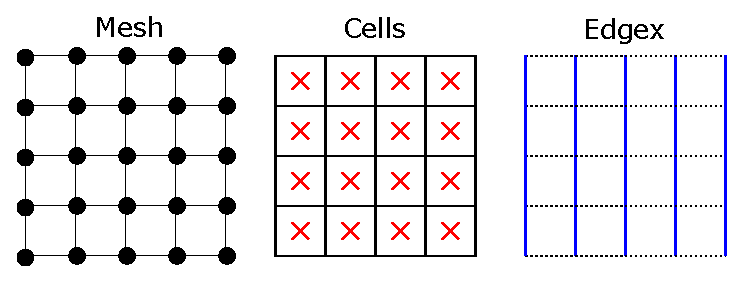
\includegraphics{./images/mesh.pdf}}
}\\
\hspace{10pt}
\subfloat[4-neighborhood stencil.\label{fig:ex1}]{
\resizebox{5cm}{!}{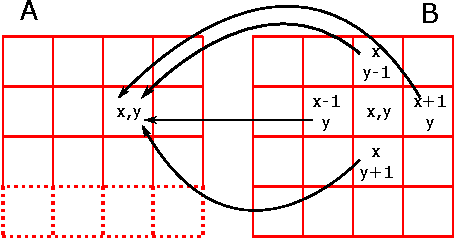
\includegraphics{./images/stencil1.pdf}}
}
\vspace{20pt}
\subfloat[4-neighborhood stencil.\label{fig:ex2}]{
\resizebox{5cm}{!}{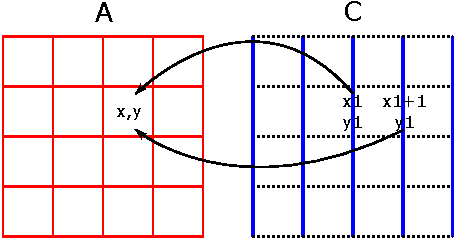
\includegraphics{./images/stencil2.pdf}}
}
\end{center}
\caption{(a) a Cartesian mesh and two kind of mesh entities, (b) an example of stencil kernel on cells, (c) an example of stencil kernel on two different entities of the mesh.}
\label{fig:gspmsp}
\end{figure}

A stencil program has been formally defined in this section. This formalism is used in the next Section to define two parallelization techniques of a multi-stencil program.

One can note that all definitions given in this section are not dependent from the topology of the mesh. This property will be kept in the rest of this paper to propose the mesh-agnostic MSL language.



%------------------------------------------------------------------------------
\section{Parallelization of Multi-Stencil Programs}
\label{sect:parallelism}
% Multi-stencil mesh-based numerical simulation can be parallelized in various ways and is an interesting kind of application to take advantage of modern heterogeneous HPC architectures, mixing clusters, multi-cores CPUs, vectorization units, GPGPU and many-core accelerators.
As previously explained, in a computation $k(S,R,(w,D),comp)$, $comp$ is not handled by MSL. As a result, in the rest of this paper, and to simplify notations, we denote the same computation $k(S,R,(w,D))$.

%------------------------------
\subsection{Data parallelism}
\label{sect:dataparal}
In a data parallelization technique, the idea is to split quantities on which the program is computed into balanced sub-parts, one for each available resource. The same sequential program can afterwards be applied on each sub-part simultaneously, with some additioinal synchronizations between resources to update the data not computed locally, and thus to guarantee a correct result.

\medskip
More formally, the data parallelization of a multi-stencil program 
\begin{equation*}
\mathcal{MSP}(\mathcal{M},\Phi,\mathcal{D},\mathcal{N},\Delta, \mathcal{S},T,\Gamma)
\end{equation*}

consists in, first, a partitioning of the mesh $\mathcal{M}$ in $p$ balanced sub-meshes (for $p$ resources) $\mathcal{M}=\{\mathcal{M}_0,\dots,\mathcal{M}_{p-1}\}$. This step can be performed by an external graph partitionner~\cite{} and is not adressed by this paper. 

As entities and quantities are mapped onto the mesh, the set of groups of mesh entities and the set of quantities $\Delta$ are partitionned the same way than the mesh: $\Phi=\{\Phi_0,\dots,\Phi_{p-1}\}$, $\Delta=\{\Delta_0,\dots,\Delta_{p-1}\}$. 

The second step of the parallelization is to identify in $\Gamma$ the needed synchronizations between resources to update data, and thus to build a new ordered list of computations $\Gamma_{sync}$.

\begin{mydef}
For $n$ the number of computations in $\Gamma$, and for $i,j$ such that $i<j<n$, a \textit{synchronization} is needed between $k_i$ and $k_j$, denoted $k_i \pprec k_j$, if $\exists (r_j,n_j) \in R_j$ such that $w_i=r_j$ and $n_j\neq identity$ ($k_j$ is a stencil computation). The quantity to synchronize is $\{w_i\}$.
\label{def:sync}
\end{mydef}

Actually, a synchronization is needed by the quantity read by a stencil computation (not local), if this quantity has been modified before, which means that it has been written before. This synchronization is needed because a neighborhood function $n \in \mathcal{N}$ of a stencil computation involves values computed on different resources.

However, as a multi-stencil program is an iterative program, computations which happen after $k_j$ at the time iteration $t$ have also been computed before $k_j$ at the previous time iteration $t-1$. For this reason another case of synchronization has to be defined.

\begin{mydef}
For $n$ the number of computations in $\Gamma$ and $j<n$, if $\exists (r_j,n_j) \in R_j$ such that $n_j\neq identity$ and for all $i<j$, $k_i \not \pprec k_j$, a \textit{synchronization} is needed between $k_l$ and $k_j$, where $j<l<n$, denoted $k_l \pprec k_j$, if $w_l=r_j$. The quantity to synchronize is $\{w_l\}$.
\label{def:sync2}
\end{mydef}

\begin{mydef}
A synchronization between two computations $k_i \pprec k_j$ is defined as a specific computation 
\begin{equation*}
k_{i,j}^{sync}(S,R,(w,D)), 
\end{equation*}
where $S=\emptyset$, $R=\{(r,n)\}=\{(w_i,n_j \in \mathcal{N}\}$, $(w,D)=(w_i,\bigcup_{\phi \in D_j} n_j(\phi)))$. In other words, $w_i$ has to be synchronized for the neighborhood $n_j$ for all entities of $D_j$.
\end{mydef}

\begin{mydef}
If $k_i \pprec k_j$, $k_j$ is replaced by the list
\begin{equation*}
[k_{i,j}^{sync}, k_j]
\end{equation*}
\end{mydef}

When data parallelism is applied, the other type of computation which is responsible for additional synchronizations is the reduction. Actually, the reduction is first applied locally on each subset of entities, on each resource. Thus, $p$ (number of resources) scalar values are obtained. For this reason, to perform the final reduction, a set of synchronizations are needed to get the final reduced scalar. As most parallelism libraries (MPI, OpenMP) already propose a reduction synchronization with its own optimizations, we simply choose to replace the reduction computation by itself anotated by $red$.

\begin{mydef}
A reduction kernel $k_j(S_j,R_j,(w_j,D_j))$, where $w$ is a scalar, is replaced by $k^{red}_j(S_j,R_j,(w_j,D_j))$. %if we denote by $w^r$, $0 \leq r<p$, the local scalar $w$ computed on the resource $r$, a reduction synchronization is defined as the specific computation 
% \begin{equation*}
% k_{j}^{sync}(S,R,(w,D),comp)
% \end{equation*}
\label{def:red}
\end{mydef}
% where, $S=\emptyset$, $R=\{(w^0,entity(w^0)) \dots (w^{p-1},entity(w^{p-1}))\}$, and $w=w_i$, $D=entity(w)=D_i$ and $comp=comp_i$.

One can notice that both types of synchronizations are performed by all resources.

\begin{mydef}
The concatenation of two ordered lists of respectively $n$ and $m$ computations $l_1=[k_i]_{0 \leq i \leq n-1}$ and $l_2=[k'_i]_{0 \leq i \leq m-1}$ is denoted $l_1 \cdot l_2$ and is equal to a new ordered list $l_3=[k_0,\dots,k_{n-1},k'_0,\dots,k'_{m-1}]$.
\end{mydef}

\begin{mydef}
From the ordered list of computation $\Gamma$, a new synchronized ordered list $\Gamma_{sync}$ is obtained from the call $\Gamma_{sync} = F_{sync}(\Gamma,0)$, where $F_{sync}$ is the recursive function defined in Algorithm~\ref{alg:sync}.
\end{mydef}

Algorithm~\ref{alg:sync} follows previous definitions to build a new ordered list which includes synchronizations. In this algorithm, lines 7 to 19 apply Definition~(\ref{def:sync}), lines 20 to 29 apply Definition~(\ref{def:sync2}), and finally lines 34 and 35 apply Definition~(\ref{def:red}). Finally, line 39 of the algorithm is the recursive call.

\begin{algorithm}
\caption{$F_{sync}$ recursive function}
\label{alg:sync}
\begin{algorithmic}[1]
\Procedure{$F_{sync}$} {$\Gamma$,$j$}
\State $k_j = \Gamma[j]$
\State $list = []$
\If {$j=|\Gamma|$}
\State return $list$
\ElsIf {$\exists (r_j,n_j) \in R_j$ such that $n_j\neq identity$}
\For {all $(r_j,n_j) \in R_j$ such that $n_j\neq identity$}
\State found = false
\For {$0 \leq i<j$}
\State $k_i = \Gamma[i]$
\If {$k_i \pprec k_j$}
\State found = true
\State $S = \emptyset$
\State $R = \{(w_i,n_j)\}$
\State $(w,D) = (w_i,\bigcup_{\phi \in D_j} n_j(\phi)))$
%\State $comp = identity$
\State $list.[k_{i;j}^{sync}(S,R,(w,D))]$%,comp)]$
\EndIf
\EndFor
\If {!found}
\For {$j<i\leq n$}
\State $k_i = \Gamma[i]$
\If {$k_i \pprec k_j$}
\State $S = \emptyset$
\State $R = \{(w_i,n_j)\}$
\State $(w,D) = (w_i,\bigcup_{\phi \in D_j} n_j(\phi)))$
%\State $comp = identity$
\State $list.[k_{i;j}^{sync}(S,R,(w,D))]$%,comp)]$
\EndIf
\EndFor
\EndIf
\State $list \cdot [k_j]$
\EndFor
\ElsIf {$w_j \in \mathcal{S}$}
\State $list.[k^{red}_j]$
\Else
\State $list.[k_j]$
\EndIf
\State return $list \cdot F_{sync}(\Gamma,j+1)$
\EndProcedure
\end{algorithmic}
\end{algorithm}


 The final step of this parallelization is to run $\Gamma_{sync}$ on each resource. Thus, for each resource $0 \leq r \leq p-1$ the multi-stencil program 
\begin{equation}
\mathcal{MSP}_r(\mathcal{M}_r,\Phi_r,\mathcal{D}_r,\mathcal{N},\Delta_r,\mathcal{S},T,\Gamma_{sync}),
\end{equation}
is performed.

\paragraph{\textbf{Example}} Figure~\ref{fig:exmsl} gives an example of a $\mathcal{MSP}$ program. From this example, the following ordered list of computation kernels can be extracted:
\begin{equation*}
\Gamma = [k_0,k_1,k_2,k_3,k_4,k_0,k_6,k_7,k_8]
\end{equation*}
From this ordered list of computation kernels $\Gamma$, and from the rest of the multi-stencil program, synchronizations can be automatically detected from the call to $F_{sync}(\Gamma,0)$ to get the synchronized ordered list of kernels:
\begin{equation}
\Gamma_{sync} = [k_0,k_{0;1}^{sync},k_1,k_2,k_3,k_{1;4}^{sync},k_4,k_0,k_6,k_7,k_{7;8}^{sync},k_8],
\label{eq:exsync}
\end{equation}
\begin{subequations}
where
\begin{align}
        k_{0;1}^{sync}=(\emptyset,\{(B,nce)\},(B,\cup_{\phi \in D_1} nce(\phi)),identity),\\
        k_{1;4}^{sync}=(\emptyset,\{(C,nec)\},(C,\cup_{\phi \in D_4} nec(\phi)),identity),\\
        k_{7;8}^{sync}=(\emptyset,\{(I,ncc)\},(I,\cup_{\phi \in D_8} ncc(\phi)),identity).
\end{align}
\end{subequations}

%------------------------------
\subsection{Hybrid parallelism}
A task parallelization technique is a technique to transform a program as a dependency graph of different tasks. A dependency graph exhibits parallel tasks, or on the contrary sequential execution of tasks. Such a dependency graph can directly be given to a dynamic scheduler, or can statically be scheduled. In this paper, we introduce task parallelism by building the dependency graph between kernels of the sequential list $\Gamma_{sync}$. Thus, as $\Gamma_{sync}$ takes into account data parallelism, we introduce hybrid parallelism.

\begin{mydef}
For two computations $k_i$ and $k_j$, with $i < j$, it is said that $k_j$ is dependant from $k_i$ with a \emph{read after write} dependency, denoted $k_i \prec_{raw} k_j$, if $\exists (r_j,n_j) \in R_j$ such that $w_i=r_j$. In this case, $k_i$ has to be computed before $k_j$.
\end{mydef}

\begin{mydef}
For two computations $k_i$ and $k_j$, with $i < j$, it is said that $k_j$ is dependant from $k_i$ with a \emph{write after write} dependency, denoted $k_i \prec_{waw} k_j$, if $w_i = w_j$ and $D_i \cap D_j \neq \emptyset$. In this case, $k_i$ also has to be computed before $k_j$.
\end{mydef}

\begin{mydef}
For two computations $k_i$ and $k_j$, with $i < j$, it is said that $k_j$ is dependant from $k_i$ with a \emph{write after read} dependency, denoted $k_i \prec_{war} k_j$, if $\exists (r_i,n_i) \in R_i$ such that $w_j=r_i$. In this case, $k_i$ also has to be computed before $k_j$ is started so that values read by $k_i$ are relevant.
\end{mydef}

Those definitions are known as \emph{data hazards classification}. However, a specific condition on the computation domain, due to the specific domain of multi-stencils, is introduced for the write after write case.

\begin{mydef}
A directed acyclic graph (DAG) $G(V,A)$ is a graph where the edges are directed from a source to a destination vertex, and where, by following edges direction, no cycle can be found from a vertex $u$ to itself. A directed edge is called an arc, and for two vertices $v,u \in V$ an arc from $u$ to $v$ is denoted $(\overset{\frown}{u,v}) \in A$.
\end{mydef}

From an ordered list of computations $\Gamma_{sync}$, a directed dependency graph $\Gamma_{dep}(V,A)$ can be built finding all pairs of computations $k_i$ and $k_j$, with $i<j$, such that $k_i \prec_{raw} k_j$ or $k_i \prec_{waw} k_j$ or $k_i \prec_{war} k_j$. 

\begin{mydef}
For two directed graphs $G(V,A)$ and $G'(V',A')$, the union $(V,A)\cup (V',A')$ is defined as the union of each set $(V\cup V', A \cup A')$.
\end{mydef}

\begin{mydef}
From the synchronized ordered list of computation kernels $\Gamma_{sync}$, the dependency graph of the computations $\Gamma_{dep}(V,A)$ is obtained from the call $F_{dep}(\Gamma_{sync},0)$, where $F_{dep}$ is the recursive function defined in Algorithm~\ref{alg:dep}.

% \begin{equation*}
% F_{dep}(\Gamma_{sync},j) = 
% \begin{cases} 	\bullet (\{\},\{\}) \mbox{ if }j=|\Gamma_{sync}|\\
% 				\bullet (k_j, \{(\overset{\frown}{k_i,k_j})\mbox{, }\forall i < j \mbox{, } k_i\prec k_j \})\\
% 				\text{ } \qquad \cup F_{dep}(\Gamma_{sync},j+1) \mbox{ if }j<|\Gamma_{sync}|
% \end{cases}
% \end{equation*}
\end{mydef}

\begin{algorithm}
\caption{$F_{dep}$ recursive function}
\label{alg:dep}
\begin{algorithmic}[1]
\Procedure{$F_{dep}$} {$\Gamma_{sync}$,$j$}
\State $k_j = \Gamma_{sync}[j]$
\If {$j=|\Gamma_{sync}|$}
\State return $(\{\},\{\})$
\ElsIf {$j<|\Gamma_{sync}|$}
\State $G=(\{\},\{\})$
\For {$0 \leq i<j$}
\State $k_i = \Gamma_{sync}[i]$
\If {$k_i \prec_{raw} k_j$ or $k_i \prec_{waw} k_j$ or $k_i \prec_{war} k_j$}
\State $G = G \cup (k_j, \{(\overset{\frown}{k_i,k_j} \})$
\EndIf
\EndFor
\State return $G \cup F_{dep}(\Gamma_{sync},j+1)$
\EndIf
\EndProcedure
\end{algorithmic}
\end{algorithm}

This constructive function is possible because the input is an ordered list. Actually, if $k_i\prec k_j$ then $i<j$. As a result, $k_i$ is already in $V$ when the arc $(\overset{\frown}{k_i,k_j})$ is built.

One can notice that $\Gamma_{dep}$ is the dependency graph of the computations of a multi-stencil program, but it only takes into account a single time iteration. A complete dependency graph of the simulation could be built. This is a possible extension of this work.

\begin{myprop}
The directed graph $\Gamma_{dep}$ is an acyclic graph.
\end{myprop}

% \begin{proof}
% $\Gamma_{dep}$ is built from $\Gamma_{sync}$ which is an ordered and sequential list of computations. Moreover, each computation of the list $\Gamma_{sync}$ is associated to a vertex of $V$, even if the same computation is represented more than once in $\Gamma_{sync}$. As a result it is not possible to go back to a previous computation and to create a cycle.
% \end{proof}

As a result of the hybrid parallelization, each resource $0 \leq r \leq p-1$ perform a multi-stencil program, defined by
\begin{equation*}
\mathcal{MSP}_r(\mathcal{M}_r,\Phi_r,\mathcal{D}_r,\mathcal{N},\Delta_r,T,\Gamma_{dep}).
\end{equation*}
The set of computations $\Gamma_{dep}$ is a dependency graph between computation kernels $k_i$ of $\Gamma$ and synchronizations of kernels added into $\Gamma_{sync}$. $\Gamma_{dep}$ can be built from the call to 
\begin{equation*}
F_{dep}(F_{sync}(\Gamma,0),0).
\end{equation*}

\paragraph{\textbf{Example}} Figure~\ref{fig:exmsl} gives an example of $\mathcal{MSP}$ program. From $\Gamma_{sync}$ that has been built in Equation~(\ref{eq:exsync}), the dependency DAG can be built. For example, as $k_0$ computes $B$ and $k_1$ reads $B$, $k_0$ and $k_1$ becomes vertices of $\Gamma_{dep}$, and an arc $(\overset{\frown}{k_0,k_1})$ is added to $\Gamma_{dep}$. The overall $\Gamma_{dep}$ built from the call to $F_{dep}(\Gamma_{sync},0)$ is drawn in Figure~\ref{fig:depdep}.
\begin{figure}[h!]
\begin{center}
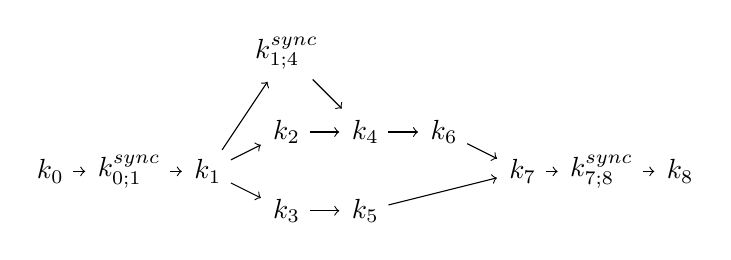
\begin{tikzpicture}[shorten >=1pt, node distance=2cm, on grid, auto]
   \node[] (c0) at (0,0) {$k_0$};
   \node[] (star1) at (1,0) {$k_{0;1}^{sync}$};
   \node[] (c1) at (2,0) {$k_1$};
   \node[] (c2) at (3,0.5) {$k_2$};
   \node[] (star4) at (3,1.5) {$k_{1;4}^{sync}$};
   \node[] (c3) at (3,-0.5) {$k_3$};
   \node[] (c4) at (4,0.5) {$k_4$};
   \node[] (c5) at (4,-0.5) {$k_5$};
   \node[] (c6) at (5,0.5) {$k_6$};
   \node[] (c7) at (6,0) {$k_7$};
   \node[] (star8) at (7,0) {$k_{7;8}^{sync}$};
   \node[] (c8) at (8,0) {$k_8$};
 
  \path[->]
    (c0) edge node {} (star1)
    (star1) edge node {} (c1)
    (c1) edge node {} (c2)
         edge node {} (c3)
         edge node {} (star4)
    (star4) edge node {} (c4)
    (c2) edge node {} (c4)
    (c4) edge node {} (c6)
    (c3) edge node {} (c5)
    (c5) edge node {} (c7)
    (c6) edge node {} (c7)
    (c7) edge node {} (star8)
    (star8) edge node {} (c8);
  \end{tikzpicture}
\caption{$\Gamma_{dep}$ of the example of program of Figure~\ref{fig:exmsl}}
\label{fig:depdep}
\end{center}
\end{figure}
%------------------------------------------------------------------------------
\section{The Multi-Stencil Language}
\label{sect:msl}
%\begin{filecontents*}{grammar.txt}
program ::= "mesh:" meshid 
            "mesh entities:" listmeshent
            "computation domains:" 
                       listcompdom
            "independent:"
                       listinde
            "data:" listdata
            listloop

listmeshent ::= meshent listmeshent |  meshent
listcompdom ::= compdom listcompdom |  compdom
compdom ::= compdomid "in" listmeshent
listinde ::= inde listinde |  inde
inde ::= compdomid "and" compdomid
listdata ::= data listdata |  data
data ::= dataid "," meshent

listloop ::= loop listloop | loop
loop ::=  "time:" iteration
          "reductions:" listred
          "computations:" listcomp
          
iteration ::= num | red
listcomp ::= comp listcomp |  comp
comp ::= dataid "[" compdomid "]=" compid "(" listdataread ")"
listred ::= red listred | red
red ::= redid "(" listdataread ")"
listdataread ::= dataread listdataread |  dataread
dataread ::= dataid "[" neighborid "]" |  dataid
\end{filecontents*}

\begin{figure}[t]
  \hspace{5mm}
  \begin{minipage}[t]{\textwidth}
    %  \subfloat[\label{fig:grammar}]
    {\lstinputlisting[basicstyle=\small,mathescape,frame=single,language=Python,numbers=left,linewidth=.87\textwidth]{grammar.txt}}   
    \caption{Grammar of the Multi-Stencil Language. \label{fig:grammar}}
  \end{minipage}
\end{figure}
%------------------------------------------------------------------------------
\section{Static Scheduling}
\label{sect:msp}
%In this section we argue that the graphs $\Gamma_{hybrid}$ or $\Gamma_{task}$, previously defined, on which an approximation will be defined, are minimal series-parallel graphs. For this reason, the structure of those graphs can be represented as binary trees of parallel and series compositions of sub-graphs, also called \emph{binary decomposition tree}~\cite{Valdes:1979:RSP:800135.804393}. First, the needed definitions on series-parallel graphs will be given...

%--------------------
\subsection{GSP and MSP classes}
A vertex $v$ of a DAG $G$ is a \emph{source} if no edge of $G$ enters $v$. Similarly, a vertex $v$ is a \emph{sink} if no edge of $G$ leaves $v$. In 1982, Valdes \& Al~\cite{Valdes:1979:RSP:800135.804393} have defined the class of minimal series-parallel DAGs (MSP).

\begin{mydef}Minimal Series Parallel
\begin{itemize}
\item The DAG having a single vertex and no edges is MSP.
\item If $G_1=(V_1,E_1)$ and $G_2=(V_2,E_2)$ are two MSP DAGs, so is either of the DAGs constructed by the following operations:
\begin{itemize}
\item Parallel composition: $G_p=(V_1\cup V_2,E_1\cup E_2)$.
\item Series composition: $G_s=(V_1\cup V_2,E_1\cup E_2\cup (N_1 \times R_2))$, where $N_1$ is the set of sinks of $G_1$ and $R_2$ is the set of sources of $G_2$.
\end{itemize}
\end{itemize}
\end{mydef}

\begin{mydef}
A DAG is \emph{General Series Parallel} (GSP) if and only if its transitive reduction is a MSP DAG.
\end{mydef}

A \emph{binary decomposition tree} is a tree having a leaf for each vertex of the MSP DAG it represents, and whose internal nodes are labelled $S$ or $P$ to indicate respectively the series or parallel composition of the MSP sub-DAGs represented by the subtrees rooted at $S$ or $P$. Figures~\ref{fig:gsp}, ~\ref{fig:msp} and~\ref{fig:t} respectively give an example of a GSP DAG, its transitive reduction which is MSP, and its tree decomposition.

\begin{figure}[h!]
\begin{center}
\subfloat[][\label{fig:gsp}]{
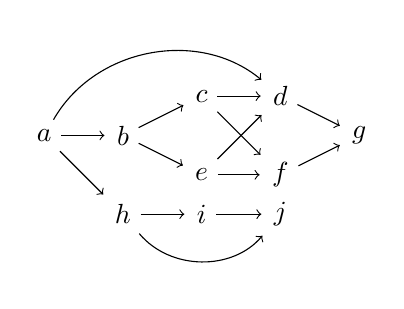
\begin{tikzpicture}[shorten >=1pt, node distance=2cm, on grid, auto]
   \node[] (a) at (0,0) {$a$};
   \node[] (b) at (1,0) {$b$};
   \node[] (c) at (2,0.5) {$c$};
   \node[] (d) at (3,0.5) {$d$};
   \node[] (e) at (2,-0.5) {$e$};
   \node[] (f) at (3,-0.5) {$f$};
   \node[] (g) at (4,0) {$g$};
   \node[] (h) at (1,-1) {$h$};
   \node[] (i) at (2,-1) {$i$};
   \node[] (j) at (3,-1) {$j$};
 
  \path[->]
    (a) edge node {} (b)
        edge [bend left=50] node [swap] {} (d)
        edge node {} (h)
    (b) edge node {} (c)
        edge node {} (e)
    (c) edge node {} (d)
        edge node {} (f)
    (e) edge node {} (d)
        edge node {} (f)
    (d) edge node {} (g)
    (f) edge node {} (g)
    (h) edge node {} (i)
        edge [bend right=50] node [swap] {} (j)
    (i) edge node {} (j);
  \end{tikzpicture}
}
\hspace{10pt}
\subfloat[][\label{fig:msp}]{
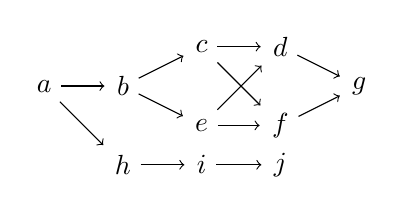
\begin{tikzpicture}[shorten >=1pt, node distance=2cm, on grid, auto]
  \node[] (a) at (0,0) {$a$};
   \node[] (b) at (1,0) {$b$};
   \node[] (c) at (2,0.5) {$c$};
   \node[] (d) at (3,0.5) {$d$};
   \node[] (e) at (2,-0.5) {$e$};
   \node[] (f) at (3,-0.5) {$f$};
   \node[] (g) at (4,0) {$g$};
   \node[] (h) at (1,-1) {$h$};
   \node[] (i) at (2,-1) {$i$};
   \node[] (j) at (3,-1) {$j$};
 
  \path[->]
    (a) edge node {} (b)
        edge node {} (h)
    (b) edge node {} (c)
        edge node {} (e)
    (c) edge node {} (d)
        edge node {} (f)
    (e) edge node {} (d)
        edge node {} (f)
    (d) edge node {} (g)
    (f) edge node {} (g)
    (h) edge node {} (i)
    (i) edge node {} (j);
  \end{tikzpicture}
}
\end{center}
\caption{(a) GSP and (b) MSP DAGs}
\label{fig:gspmsp}
\end{figure}

\begin{figure}[h!]
\begin{center}
\begin{tikzpicture}[shorten >=1pt, node distance=2cm, on grid, auto]
   \node[] (S1) at (0,0) {$\mathcal{S}$};
   \node[] (P1) at (0.5,1) {$\mathcal{P}$};
   \node[] (a) at (-0.5,1) {$a$};
   \node[] (S2) at (-1,2) {$\mathcal{S}$}; %+1
   \node[] (S3) at (2,2) {$\mathcal{S}$}; %-1
   \node[] (b) at (-2,3) {$b$};
   \node[] (S4) at (0,3) {$\mathcal{S}$};
   \node[] (P2) at (-1,4) {$\mathcal{P}$};
   \node[] (g) at (1,4) {$g$};
   \node[] (S5) at (-2,5) {$\mathcal{S}$};
   \node[] (S6) at (0,5) {$\mathcal{S}$};
   \node[] (c) at (-2.5,6) {$c$};
   \node[] (d) at (-1.5,6) {$d$};
   \node[] (e) at (-0.5,6) {$e$};
   \node[] (f) at (0.5,6) {$f$};
   
   \node[] (h) at (1,3) {$h$};
   \node[] (S7) at (3,3) {$\mathcal{S}$};
   \node[] (i) at (2.5,4) {$i$};
   \node[] (j) at (3.5,4) {$j$};
 
  \path[->]
    (S1) edge node {} (a)
          edge node {} (P1)
    (P1) edge node {} (S2)
          edge node {} (S3)
    (S2) edge node {} (b)
        edge node {} (S4)
    (S4) edge node {} (P2)
          edge node {} (g)
    (P2) edge node {} (S5)
          edge node {} (S6)
    (S5) edge node {} (c)
          edge node {} (d)
    (S6) edge node {} (e)
          edge node {} (f)
    (S3) edge node {} (h)
         edge node {} (S7)
    (S7) edge node {} (i)
          edge node {} (j);
  \end{tikzpicture}
  \caption{Binary decomposition tree of the MSP of Figure~\ref{fig:msp}}
  \label{fig:t}
\end{center}
\end{figure}

Valdes \& Al~\cite{Valdes:1979:RSP:800135.804393} have also proposed a linear algorithm to know if a DAG is MSP and, if it is, to decompose it to its associated binary decomposition tree. This algorithm is based on the duality of the class of MSP DAGs, with the class of \emph{Two Terminal Series Parallel} DAGs (TTSP) from which a binary tree decomposition can be performed in linear time. However, in this paper we are interested in DAGs that we already know as MSP. Thus, we only give the needed definitions to understand the binary decomposition algorithm, and not the recognition algorithm. To let the reader understand this algorithm, which is modified in this work, the needed definitions are given. 
%  Other algorithms have also been proposed, all of them in linear time~\cite{Schoenmakers95anew}.

\begin{mydef}
The \emph{line digraph} of a digraph $G$ is a digraph $L(G)$ that has:
\begin{itemize}
\item a vertex $f(e)$ for each edge $e$ of $G$; and
\item an edge $(f(e_1),f(e_2))$ for each pair of edges of $G$ of the form $e_1=(u,v)$, $e_2=(v,w)$.
\end{itemize}
\end{mydef}

\begin{mydef}Two Terminal Series Parallel
\begin{itemize}
\item A digraph consisting of two vertices joined by a single edge is TTSP.
\item If $G_1$ and $G_2$ are TTSP digraphs, so is the digraph obtained by either of the following operations:
\begin{itemize}
\item \emph{Two terminal parallel composition}: identify the sourc of $G_1$ with the source of $G_2$ and the sink of $G_1$ with the sink of $G_2$.
\item \emph{Two terminal series composition}: identify the sink of $G_1$ with the source of $G_2$.
\end{itemize}
\end{itemize}
\end{mydef}

\begin{myth}
If the DAG $G$ is a MSP graph, its \emph{inverse line DAG} $L^{-1}(G)$ is TTSP.
\end{myth}

It has to be indicate that for a DAG $G$, $L^{-1}(G)$ is not unique. Thus, in the work of Valdes \& Al, and in this work, $L^{-1}(G)$ will refer to the unique digraph having a single source and a single sink whose line digraph is $L(L^{-1}(G))=G$.

The binary decomposition tree algorithm is based on the fact that the decomposition can be obtained as a byproduct of a reduction process. In order to obtain the decomposition, Valdes \& Al associate a label with each edge of the digraph being reduced. Initially the label of each edge is a trivial binary tree consisting of a single node. As the reduction process introduces new edges the rules of Figure~\ref{fig:rules} are used to compute the binary trees used to label them. The algorithm ends when the TTSP graph is reduced to its minimum, i.e.\ two vertices and a single edge between them.

\begin{figure}[h!]
\captionsetup[subfigure]{labelformat=empty}
\begin{center}
%FIRST RULE
\subfloat[]{
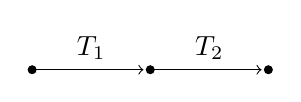
\begin{tikzpicture}[shorten >=1pt, node distance=2cm, on grid, auto]
   \node[circle,draw=black,fill=black,scale=0.3] (x) at (0,0) {};
   \node[circle,draw=black,fill=black,scale=0.3] (y) at (1.5,0) {};
   \node[circle,draw=black,fill=black,scale=0.3] (z) at (3,0) {};
 
  \path[->]
    (x) edge node [above] {$T_1$} (y)
    (y) edge node [above] {$T_2$} (z);
  \end{tikzpicture}
  }
\hspace{50pt}
%ARROW
\subfloat[]{
$\Rightarrow$
}
\hspace{50pt}
%SECOND RULE
\subfloat[]{
\begin{tikzpicture}[shorten >=1pt, node distance=2cm, on grid, auto]
   \node[circle,draw=black,fill=black,scale=0.3] (x) at (0,0) {};
   \node[circle,draw=black,fill=black,scale=0.3] (y) at (3,0) {};
   \node[] (s) at (1.5,0.5) {$\mathcal{S}$};
   \node[] (t1) at (1,1.5) {$T_1$};
   \node[] (t2) at (2,1.5) {$T_2$};
 
  \path[->]
    (x) edge node {} (y)
    (s) edge node {} (t1)
        edge node {} (t2);
  \end{tikzpicture}
}
\\
\subfloat[]{
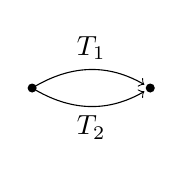
\begin{tikzpicture}[shorten >=1pt, node distance=2cm, on grid, auto]
   \node[circle,draw=black,fill=black,scale=0.3] (x) at (0,0) {};
   \node[circle,draw=black,fill=black,scale=0.3] (y) at (1.5,0) {};
 
  \path[->]
    (x) edge [bend left] node [above] {$T_1$} (y)
        edge [bend right] node [below] {$T_2$} (y);
  \end{tikzpicture}
  }
\hspace{50pt}
\subfloat[]{
$\Rightarrow$
}
\hspace{50pt}
\subfloat[]{
\begin{tikzpicture}[shorten >=1pt, node distance=2cm, on grid, auto]
   \node[circle,draw=black,fill=black,scale=0.3] (x) at (0,0) {};
   \node[circle,draw=black,fill=black,scale=0.3] (y) at (3,0) {};
   \node[] (p) at (1.5,0.5) {$\mathcal{P}$};
   \node[] (t1) at (1,1.5) {$T_1$};
   \node[] (t2) at (2,1.5) {$T_2$};
 
  \path[->]
    (x) edge node {} (y)
    (p) edge node {} (t1)
        edge node {} (t2);
  \end{tikzpicture}
}
\caption{Reduction rules of the decomposition tree algorithm.}
\label{fig:rules}
\end{center}
\end{figure}

Finally, Valdes \& Al~\cite{Valdes:1979:RSP:800135.804393} have identify a forbidden shape, or subgraph, called $N$ and represented in Figure~\ref{fig:n}, such that 

\begin{myth}
A DAG $G$ is GSP if and only if its transitive closure does not contain $N$ as a subgraph.
\end{myth}

\begin{figure}[h!]
\begin{center}
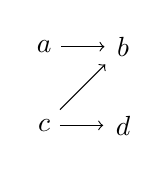
\begin{tikzpicture}[shorten >=1pt, node distance=2cm, on grid, auto]
   \node[] (a) at (0,0) {$a$};
   \node[] (b) at (1,0) {$b$};
   \node[] (c) at (0,-1) {$c$};
   \node[] (d) at (1,-1) {$d$};
 
  \path[->]
    (a) edge node {} (b)
    (c) edge node {} (b)
        edge node {} (d);
  \end{tikzpicture}
  \caption{Forbidden $N$ subgraph shape for a DAG to be GSP.}
  \label{fig:n}
\end{center}
\end{figure}

%------------------
\subsection{Multi-stencil programs.}
We are interested in GSP and MSP classes of graphs to be able to represent computations of a multi-stencil program as a set of sequences and parallel executions. Actually, such a representation can directly be dumped to a parallel language, in which \emph{sequence} of instructions and \emph{parallel} execution of instructions are defined. Series-parallel trees can also be used as input of scheduling optimizations~\cite{Finta1996323,Wang20082684} to improve task parallelism efficiency, which opens more perspectives to this work. Finally, in this paper is presented that such a series-parallel representation can also be dumped to component models by defining specific control components. Thus, the proposed DSL inheritates software engineering advantages of component models, such as code re-use, productivity and maintainability.

Returning back to the parallelization formalism of Section~\ref{}, two important steps have to be performed to make $\Gamma_{hybrid}$ a MSP graph:
\begin{itemize}
\item transitive reduction,
\item deletion of the forbidden $N$ shape.
\end{itemize}

The transitive reduction has already been applied on $\Gamma_{hybrid}$ by the transitivity of the relation $\blacktriangleleft$. However, even by applying this transitive reduction it is possible to obtain a DAG which is not MSP. Actually, it is possible in a multi-stencil program to have a set of computations such that their dependencies form the forbidden $N$ subgraph. For example, if $c_0$, $c_1$, $c_2$ and $c_3$ are computations of a $\mathcal{MSP}$ such that $c_0 \prec c_1$, $c_2 \prec c_1$ and $c_2 \prec c_3$, the \emph{zigzag} relation $c_0 \prec c_1 \succ c_2 \prec c_3$ which form a forbidden subgraph of MSP DAGs is found in $\Gamma_{hybrid}$. For this reason, we have made the choice to over-constrain such a case by adding the relation $c_0 \prec c_3$ such that a complete graph is created and can be translated to a series-parallel decomposition as illustrated in Figure~\ref{fig:allover}.

\begin{figure}[h!]
\begin{center}
\subfloat[][Over-constraint on the forbidden $N$ shape.\label{fig:over}]{
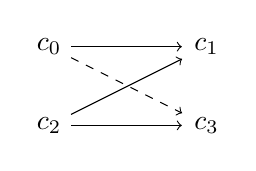
\begin{tikzpicture}[shorten >=1pt, node distance=2cm, on grid, auto]
   \node[] (c0) at (0,0) {$c_0$};
   \node[] (c1) at (2,0) {$c_1$};
   \node[] (c2) at (0,-1) {$c_2$};
   \node[] (c3) at (2,-1) {$c_3$};
 
  \path[->]
    (c0) edge node {} (c1)
          edge [dashed] node [swap] {} (c3)
    (c2) edge node {} (c1)
        edge node {} (c3);
  \end{tikzpicture}
}
\hspace{50pt}
\subfloat[][Series-parallel tree associated to the over-constraint\label{fig:treeover}]{
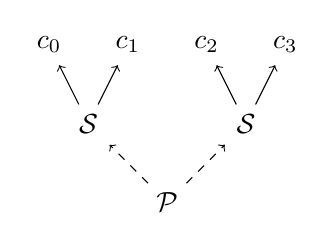
\begin{tikzpicture}[shorten >=1pt, node distance=2cm, on grid, auto]
   \node[] (P1) at (0,0) {$\mathcal{P}$};
   \node[] (S1) at (-1,1) {$\mathcal{S}$};
   \node[] (S2) at (1,1) {$\mathcal{S}$};
   \node[] (c0) at (-1.5,2) {$c_0$};
   \node[] (c1) at (-0.5,2) {$c_1$};
   \node[] (c2) at (0.5,2) {$c_2$};
   \node[] (c3) at (1.5,2) {$c_3$};
 
  \path[->]
    (P1) edge [dashed] node [swap] {} (S1)
          edge [dashed] node [swap] {} (S2)
    (S1) edge node {} (c0)
          edge node {} (c1)
    (S2) edge node {} (c2)
        edge node {} (c3);
  \end{tikzpicture}
}
\caption{Deletion of forbidden subgraphs.}
\label{fig:allover}
\end{center}
\end{figure}

This approximation on the dependencies is acceptable for multi-stencil programs, first because it rarely appends, second because of the relative homogeneity of computations. Actually, all computations, except the ones on the physical border of the domain, are performed on an entire domain of the mesh, and as a computation performs a single quantity at a time ($w_i$ of $c_i$ is a singleton), the amount of arithmetic operations in a computation are quite homogeneous.

After these over-constraints are applied, $\Gamma_{hybrid}$ is a MSP DAG. As a result, the binary tree decomposition algorithm of Valdes \& Al can be applied on $\Gamma_{hybrid}$. However, because of updated-computations inserted in $\Gamma_{data}$, we have to define additional reduction rules for the algorithm. For an updated-computation $c^*_j(c_j,\text{update}(\{w_i\text{, }\forall i\text{ }c_i \prec c_j\}))$, we define $*_j$ as the update needed by $c_j$, $*_j = \text{update}(\{w_i\text{, }\forall i\text{ }c_i \prec c_j\})$. As a result, the updated-computation $c^*_j$ is defined by $c^*_j(c_j,*_j)$. The initial label of the edges of the graph to reduce are the computations of the multi-stencil program. Four new rules are needed to perform the binary tree decomposition of $\Gamma_{hybrid}$ and are defined in Figure~\ref{fig:newrules}.

\begin{figure}[h!]
\captionsetup[subfigure]{labelformat=empty}
\begin{center}
%FIRST RULE
\subfloat[]{
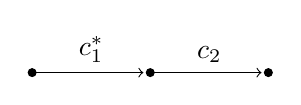
\begin{tikzpicture}[shorten >=1pt, node distance=2cm, on grid, auto]
   \node[circle,draw=black,fill=black,scale=0.3] (x) at (0,0) {};
   \node[circle,draw=black,fill=black,scale=0.3] (y) at (1.5,0) {};
   \node[circle,draw=black,fill=black,scale=0.3] (z) at (3,0) {};
 
  \path[->]
    (x) edge node [above] {$c_1^*$} (y)
    (y) edge node [above] {$c_2$} (z);
  \end{tikzpicture}
  }
\hspace{50pt}
%ARROW
\subfloat[]{
$\Rightarrow$
}
\hspace{50pt}
%TRANSFORMATION
\subfloat[]{
\begin{tikzpicture}[shorten >=1pt, node distance=2cm, on grid, auto]
   \node[circle,draw=black,fill=black,scale=0.3] (x) at (0,0) {};
   \node[circle,draw=black,fill=black,scale=0.3] (y) at (3,0) {};
   \node[] (s1) at (1.5,0.5) {$\mathcal{S}$};
   \node[] (s2) at (1,1.5) {$\mathcal{S}$};
   \node[] (star) at (0.5,2.5) {$*_1$};
   \node[] (t1) at (1.5,2.5) {$c_1$};
   \node[] (t2) at (2,1.5) {$c_2$};
 
  \path[->]
    (x) edge node {} (y)
    (s1) edge node {} (s2)
        edge node {} (t2)
    (s2) edge node {} (star)
         edge node {} (t1);
  \end{tikzpicture}
}
\\
%SECOND RULE
%FIRST RULE
\subfloat[]{
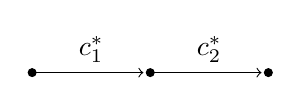
\begin{tikzpicture}[shorten >=1pt, node distance=2cm, on grid, auto]
   \node[circle,draw=black,fill=black,scale=0.3] (x) at (0,0) {};
   \node[circle,draw=black,fill=black,scale=0.3] (y) at (1.5,0) {};
   \node[circle,draw=black,fill=black,scale=0.3] (z) at (3,0) {};
 
  \path[->]
    (x) edge node [above] {$c_1^*$} (y)
    (y) edge node [above] {$c_2^*$} (z);
  \end{tikzpicture}
  }
\hspace{50pt}
%ARROW
\subfloat[]{
$\Rightarrow$
}
\hspace{50pt}
%TRANSFORMATION
\subfloat[]{
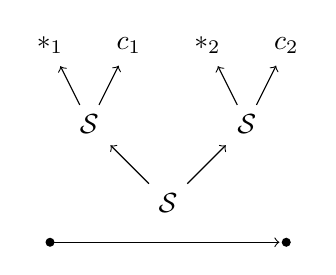
\begin{tikzpicture}[shorten >=1pt, node distance=2cm, on grid, auto]
   \node[circle,draw=black,fill=black,scale=0.3] (x) at (0,0) {};
   \node[circle,draw=black,fill=black,scale=0.3] (y) at (3,0) {};
   \node[] (s1) at (1.5,0.5) {$\mathcal{S}$};
   \node[] (s2) at (0.5,1.5) {$\mathcal{S}$};
   \node[] (s3) at (2.5,1.5) {$\mathcal{S}$};
   \node[] (star1) at (0,2.5) {$*_1$};
   \node[] (t1) at (1,2.5) {$c_1$};
   \node[] (star2) at (2,2.5) {$*_2$};
   \node[] (t2) at (3,2.5) {$c_2$};
 
  \path[->]
    (x) edge node {} (y)
    (s1) edge node {} (s2)
        edge node {} (s3)
    (s2) edge node {} (star1)
         edge node {} (t1)
    (s3) edge node {} (star2)
         edge node {} (t2);
  \end{tikzpicture}
}
\\
%THIRD RULE
\subfloat[]{
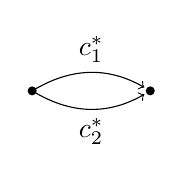
\begin{tikzpicture}[shorten >=1pt, node distance=2cm, on grid, auto]
   \node[circle,draw=black,fill=black,scale=0.3] (x) at (0,0) {};
   \node[circle,draw=black,fill=black,scale=0.3] (y) at (1.5,0) {};
 
  \path[->]
    (x) edge [bend left] node [above] {$c_1^*$} (y)
        edge [bend right] node [below] {$c_2^*$} (y);
  \end{tikzpicture}
  }
\hspace{50pt}
%ARROW
\subfloat[]{
$\Rightarrow$
}
\hspace{50pt}
%TRANSFORMATION
\subfloat[]{
\begin{tikzpicture}[shorten >=1pt, node distance=2cm, on grid, auto]
   \node[circle,draw=black,fill=black,scale=0.3] (x) at (0,0) {};
   \node[circle,draw=black,fill=black,scale=0.3] (y) at (3,0) {};
   \node[] (p) at (1.5,0.5) {$\mathcal{P}$};
   \node[] (s) at (1,1.5) {$\mathcal{S}$};
   \node[] (star) at (0.5,2.5) {$*_1$};
   \node[] (t1) at (1.5,2.5) {$c_1$};
   \node[] (t2) at (2,1.5) {$c_2$};
 
  \path[->]
    (x) edge node {} (y)
    (p) edge node {} (s)
        edge node {} (t2)
    (s) edge node {} (star)
        edge node {} (t1);
  \end{tikzpicture}
}
\\
%FOURTH RULE
\subfloat[]{
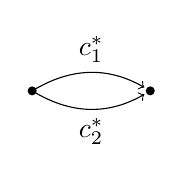
\begin{tikzpicture}[shorten >=1pt, node distance=2cm, on grid, auto]
   \node[circle,draw=black,fill=black,scale=0.3] (x) at (0,0) {};
   \node[circle,draw=black,fill=black,scale=0.3] (y) at (1.5,0) {};
 
  \path[->]
    (x) edge [bend left] node [above] {$c_1^*$} (y)
        edge [bend right] node [below] {$c_2^*$} (y);
  \end{tikzpicture}
  }
\hspace{50pt}
%ARROW
\subfloat[]{
$\Rightarrow$
}
\hspace{50pt}
%TRANSFORMATION
\subfloat[]{
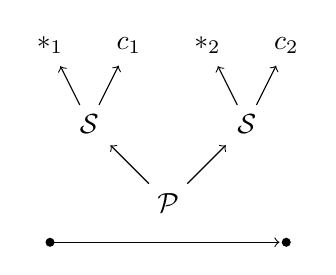
\begin{tikzpicture}[shorten >=1pt, node distance=2cm, on grid, auto]
   \node[circle,draw=black,fill=black,scale=0.3] (x) at (0,0) {};
   \node[circle,draw=black,fill=black,scale=0.3] (y) at (3,0) {};
   \node[] (p) at (1.5,0.5) {$\mathcal{P}$};
   \node[] (s2) at (0.5,1.5) {$\mathcal{S}$};
   \node[] (s3) at (2.5,1.5) {$\mathcal{S}$};
   \node[] (star1) at (0,2.5) {$*_1$};
   \node[] (t1) at (1,2.5) {$c_1$};
   \node[] (star2) at (2,2.5) {$*_2$};
   \node[] (t2) at (3,2.5) {$c_2$};
 
  \path[->]
    (x) edge node {} (y)
    (p) edge node {} (s2)
        edge node {} (s3)
    (s2) edge node {} (star1)
         edge node {} (t1)
    (s3) edge node {} (star2)
         edge node {} (t2);
  \end{tikzpicture}
}
\caption{Reduction rules of the decomposition tree algorithm.}
\label{fig:newrules}
\end{center}
\end{figure}

Using those additional reduction rules, the binary series-parallel tree decomposition can be computed in linear time. A complete example of reduction is given in Figure~\ref{fig:example}. The initial $\Gamma_{hybrid}$ DAG and its inverse line graph are given first, followed by the set of reductions. The label of the final single edge corresponds to the binary tree decomposition of the initial $\Gamma_{hybrid}$ graph. 

%====BIG EXAMPLE
\begin{figure}[ht!]
\begin{center}
% INITIAL GRAPH
\subfloat[]{
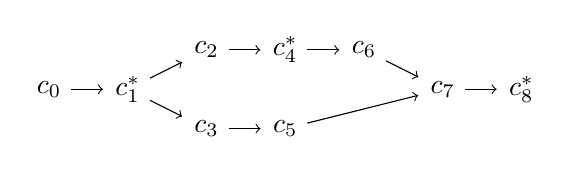
\begin{tikzpicture}[shorten >=1pt, node distance=2cm, on grid, auto]
   \node[] (c0) at (0,0) {$c_0$};
   \node[] (c1) at (1,0) {$c_1^*$};
   \node[] (c2) at (2,0.5) {$c_2$};
   \node[] (c3) at (2,-0.5) {$c_3$};
   \node[] (c4) at (3,0.5) {$c_4^*$};
   \node[] (c5) at (3,-0.5) {$c_5$};
   \node[] (c6) at (4,0.5) {$c_6$};
   \node[] (c7) at (5,0) {$c_7$};
   \node[] (c8) at (6,0) {$c_8^*$};
 
  \path[->]
    (c0) edge node {} (c1)
    (c1) edge node {} (c2)
         edge node {} (c3)
    (c2) edge node {} (c4)
    (c4) edge node {} (c6)
    (c3) edge node {} (c5)
    (c5) edge node {} (c7)
    (c6) edge node {} (c7)
    (c7) edge node {} (c8);
  \end{tikzpicture}
}
\\
% INVERSE LINE GRAPH
\subfloat[]{
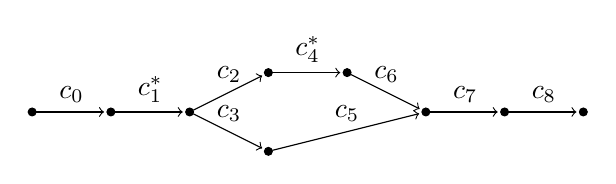
\begin{tikzpicture}[shorten >=1pt, node distance=2cm, on grid, auto]
   \node[circle,draw=black,fill=black,scale=0.3] (c0s) at (0,0) {};
   \node[circle,draw=black,fill=black,scale=0.3] (c0d) at (1,0) {};
   \node[circle,draw=black,fill=black,scale=0.3] (c1d) at (2,0) {};
   \node[circle,draw=black,fill=black,scale=0.3] (c2d) at (3,0.5) {};
   \node[circle,draw=black,fill=black,scale=0.3] (c3d) at (3,-0.5) {};
   \node[circle,draw=black,fill=black,scale=0.3] (c4d) at (4,0.5) {};
   \node[circle,draw=black,fill=black,scale=0.3] (c6d) at (5,0) {};
   \node[circle,draw=black,fill=black,scale=0.3] (c7d) at (6,0) {};
   \node[circle,draw=black,fill=black,scale=0.3] (c8d) at (7,0) {};
 
  \path[->]
    (c0s) edge node [above] {$c_0$} (c0d)
    (c0d) edge node [above] {$c_1^*$} (c1d)
    (c1d) edge node [above] {$c_2$} (c2d)
          edge node [above] {$c_3$} (c3d)
    (c2d) edge node [above] {$c_4^*$} (c4d)
    (c4d) edge node [above] {$c_6$} (c6d)
    (c6d) edge node [above] {$c_7$} (c7d)
    (c7d) edge node [above] {$c_8$} (c8d)
    (c3d) edge node [above] {$c_5$} (c6d);
  \end{tikzpicture}
}
\\
% TRANSFORMATIONS
\subfloat[]{
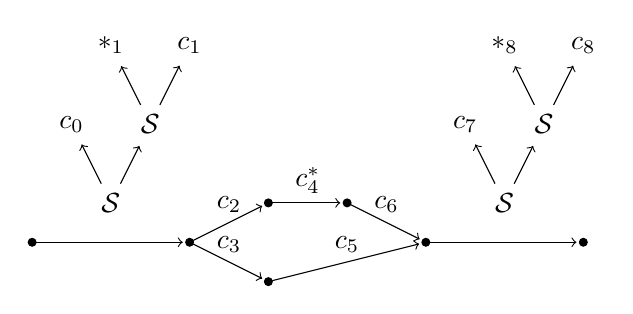
\begin{tikzpicture}[shorten >=1pt, node distance=2cm, on grid, auto]
   \node[circle,draw=black,fill=black,scale=0.3] (c0s) at (0,0) {};
   \node[circle,draw=black,fill=black,scale=0.3] (c1d) at (2,0) {};
   \node[circle,draw=black,fill=black,scale=0.3] (c2d) at (3,0.5) {};
   \node[circle,draw=black,fill=black,scale=0.3] (c3d) at (3,-0.5) {};
   \node[circle,draw=black,fill=black,scale=0.3] (c4d) at (4,0.5) {};
   \node[circle,draw=black,fill=black,scale=0.3] (c6d) at (5,0) {};
   \node[circle,draw=black,fill=black,scale=0.3] (c8d) at (7,0) {};

   %reduction c0 c1
   \node[] (s1) at (1,0.5) {$\mathcal{S}$};
   \node[] (c0) at (0.5,1.5) {$c_0$};
   \node[] (s2) at (1.5,1.5) {$\mathcal{S}$};
   \node[] (star1) at (1,2.5) {$*_1$};
   \node[] (c1) at (2,2.5) {$c_1$};

   %reduction c7 c8
   \node[] (s3) at (6,0.5) {$\mathcal{S}$};
   \node[] (c7) at (5.5,1.5) {$c_7$};
   \node[] (s4) at (6.5,1.5) {$\mathcal{S}$};
   \node[] (star8) at (6,2.5) {$*_8$};
   \node[] (c8) at (7,2.5) {$c_8$};
 
  \path[->]
    (c0s) edge node {} (c1d)
    (c1d) edge node [above] {$c_2$} (c2d)
          edge node [above] {$c_3$} (c3d)
    (c2d) edge node [above] {$c_4^*$} (c4d)
    (c4d) edge node [above] {$c_6$} (c6d)
    (c6d) edge node [above] {} (c8d)
    (c3d) edge node [above] {$c_5$} (c6d)

    %reduction c0 c1
    (s1) edge node {} (c0)
         edge node {} (s2)
    (s2) edge node {} (star1)
         edge node {} (c1)
    %reduction c7 c8
    (s3) edge node {} (c7)
         edge node {} (s4)
    (s4) edge node {} (star8)
         edge node {} (c8);
  \end{tikzpicture}
}
\\
\subfloat[]{
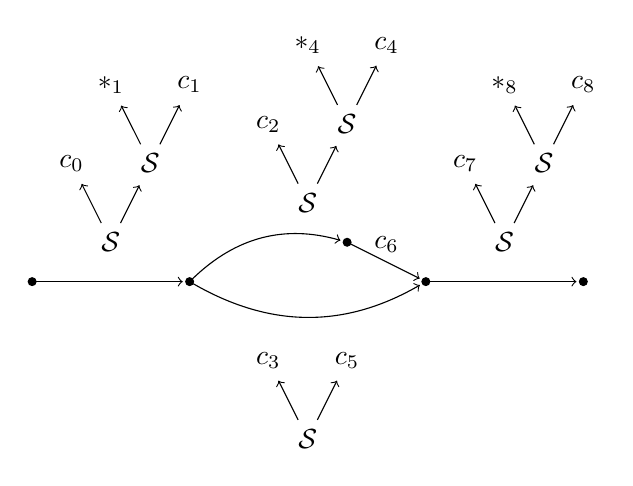
\begin{tikzpicture}[shorten >=1pt, node distance=2cm, on grid, auto]
   \node[circle,draw=black,fill=black,scale=0.3] (c0s) at (0,0) {};
   \node[circle,draw=black,fill=black,scale=0.3] (c1d) at (2,0) {};
   \node[circle,draw=black,fill=black,scale=0.3] (c4d) at (4,0.5) {};
   \node[circle,draw=black,fill=black,scale=0.3] (c6d) at (5,0) {};
   \node[circle,draw=black,fill=black,scale=0.3] (c8d) at (7,0) {};

   %reduction c0 c1
   \node[] (s1) at (1,0.5) {$\mathcal{S}$};
   \node[] (c0) at (0.5,1.5) {$c_0$};
   \node[] (s2) at (1.5,1.5) {$\mathcal{S}$};
   \node[] (star1) at (1,2.5) {$*_1$};
   \node[] (c1) at (2,2.5) {$c_1$};

   %reduction c7 c8
   \node[] (s3) at (6,0.5) {$\mathcal{S}$};
   \node[] (c7) at (5.5,1.5) {$c_7$};
   \node[] (s4) at (6.5,1.5) {$\mathcal{S}$};
   \node[] (star8) at (6,2.5) {$*_8$};
   \node[] (c8) at (7,2.5) {$c_8$};

   %reduction c3 c5
   \node[] (s5) at (3.5,-2) {$\mathcal{S}$};
   \node[] (c3) at (3,-1) {$c_3$};
   \node[] (c5) at (4,-1) {$c_5$};

   %reduction c2 c4
   \node[] (s6) at (3.5,1) {$\mathcal{S}$};
   \node[] (c2) at (3,2) {$c_2$};
   \node[] (s7) at (4,2) {$\mathcal{S}$};
   \node[] (star4) at (3.5,3) {$*_4$};
   \node[] (c4) at (4.5,3) {$c_4$};
 
  \path[->]
    (c0s) edge node {} (c1d)
    (c1d) edge [bend left] node [above] {} (c4d)
    (c4d) edge node [above] {$c_6$} (c6d)
    (c6d) edge node [above] {} (c8d)
    (c1d) edge [bend right] node [above] {} (c6d)

    %reduction c0 c1
    (s1) edge node {} (c0)
         edge node {} (s2)
    (s2) edge node {} (star1)
         edge node {} (c1)
    %reduction c7 c8
    (s3) edge node {} (c7)
         edge node {} (s4)
    (s4) edge node {} (star8)
         edge node {} (c8)

    %reduction c3 c5
    (s5) edge node {} (c3)
         edge node {} (c5)

    %reduction c7 c8
    (s6) edge node {} (c2)
         edge node {} (s7)
    (s7) edge node {} (star4)
         edge node {} (c4);
  \end{tikzpicture}
}
\end{center}
\caption{Big example}
\label{fig:example}
\end{figure}

\begin{figure}[ht!]
\ContinuedFloat
\begin{center}
\subfloat[]{
\begin{tikzpicture}[shorten >=1pt, node distance=2cm, on grid, auto]
   \node[circle,draw=black,fill=black,scale=0.3] (c0s) at (0,0) {};
   \node[circle,draw=black,fill=black,scale=0.3] (c1d) at (2,0) {};
   \node[circle,draw=black,fill=black,scale=0.3] (c6d) at (5,0) {};
   \node[circle,draw=black,fill=black,scale=0.3] (c8d) at (7,0) {};

   %reduction c0 c1
   \node[] (s1) at (1,0.5) {$\mathcal{S}$};
   \node[] (c0) at (0.5,1.5) {$c_0$};
   \node[] (s2) at (1.5,1.5) {$\mathcal{S}$};
   \node[] (star1) at (1,2.5) {$*_1$};
   \node[] (c1) at (2,2.5) {$c_1$};

   %reduction c7 c8
   \node[] (s3) at (6,0.5) {$\mathcal{S}$};
   \node[] (c7) at (5.5,1.5) {$c_7$};
   \node[] (s4) at (6.5,1.5) {$\mathcal{S}$};
   \node[] (star8) at (6,2.5) {$*_8$};
   \node[] (c8) at (7,2.5) {$c_8$};

   %reduction c3 c5
   \node[] (s5) at (3.5,-2) {$\mathcal{S}$};
   \node[] (c3) at (3,-1) {$c_3$};
   \node[] (c5) at (4,-1) {$c_5$};

   %reduction c2 c6
   \node[] (s8) at (3.5,1) {$\mathcal{S}$};
   \node[] (c6) at (4,2) {$c_6$};
   \node[] (s6) at (3,2) {$\mathcal{S}$};
   \node[] (c2) at (2.5,3) {$c_2$};
   \node[] (s7) at (3.5,3) {$\mathcal{S}$};
   \node[] (star4) at (3,4) {$*_4$};
   \node[] (c4) at (4,4) {$c_4$};
 
  \path[->]
    (c0s) edge node {} (c1d)
    (c1d) edge [bend left] node [above] {} (c6d)
    (c6d) edge node [above] {} (c8d)
    (c1d) edge [bend right] node [above] {} (c6d)

    %reduction c0 c1
    (s1) edge node {} (c0)
         edge node {} (s2)
    (s2) edge node {} (star1)
         edge node {} (c1)
    %reduction c7 c8
    (s3) edge node {} (c7)
         edge node {} (s4)
    (s4) edge node {} (star8)
         edge node {} (c8)

    %reduction c3 c5
    (s5) edge node {} (c3)
         edge node {} (c5)

    %reduction c2 c6
    (s8) edge node {} (s6)
         edge node {} (c6)
    (s6) edge node {} (c2)
         edge node {} (s7)
    (s7) edge node {} (star4)
         edge node {} (c4);
  \end{tikzpicture}
}
\\
\subfloat[]{
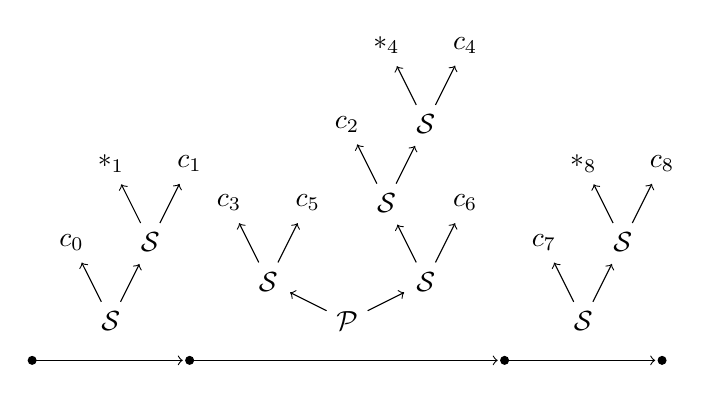
\begin{tikzpicture}[shorten >=1pt, node distance=2cm, on grid, auto]
   \node[circle,draw=black,fill=black,scale=0.3] (c0s) at (0,0) {};
   \node[circle,draw=black,fill=black,scale=0.3] (c1d) at (2,0) {};
   \node[circle,draw=black,fill=black,scale=0.3] (c6d) at (6,0) {};
   \node[circle,draw=black,fill=black,scale=0.3] (c8d) at (8,0) {};

   %reduction c0 c1
   \node[] (s1) at (1,0.5) {$\mathcal{S}$};
   \node[] (c0) at (0.5,1.5) {$c_0$};
   \node[] (s2) at (1.5,1.5) {$\mathcal{S}$};
   \node[] (star1) at (1,2.5) {$*_1$};
   \node[] (c1) at (2,2.5) {$c_1$};

   %reduction c7 c8
   \node[] (s3) at (7,0.5) {$\mathcal{S}$};
   \node[] (c7) at (6.5,1.5) {$c_7$};
   \node[] (s4) at (7.5,1.5) {$\mathcal{S}$};
   \node[] (star8) at (7,2.5) {$*_8$};
   \node[] (c8) at (8,2.5) {$c_8$};

   %reduction c2 c4 c6 c3 c5
   \node[] (p1) at (4,0.5) {$\mathcal{P}$};
   \node[] (s5) at (3,1) {$\mathcal{S}$};
   \node[] (c3) at (2.5,2) {$c_3$};
   \node[] (c5) at (3.5,2) {$c_5$};
   \node[] (s8) at (5,1) {$\mathcal{S}$};
   \node[] (c6) at (5.5,2) {$c_6$};
   \node[] (s6) at (4.5,2) {$\mathcal{S}$};
   \node[] (c2) at (4,3) {$c_2$};
   \node[] (s7) at (5,3) {$\mathcal{S}$};
   \node[] (star4) at (4.5,4) {$*_4$};
   \node[] (c4) at (5.5,4) {$c_4$};
 
  \path[->]
    (c0s) edge node {} (c1d)
    (c1d) edge node [above] {} (c6d)
    (c6d) edge node [above] {} (c8d)

    %reduction c0 c1
    (s1) edge node {} (c0)
         edge node {} (s2)
    (s2) edge node {} (star1)
         edge node {} (c1)
    %reduction c7 c8
    (s3) edge node {} (c7)
         edge node {} (s4)
    (s4) edge node {} (star8)
         edge node {} (c8)

    %reduction c2 c4 c6 c3 c5
    (p1) edge node {} (s5)
         edge node {} (s8)
    (s5) edge node {} (c3)
         edge node {} (c5)
    (s8) edge node {} (s6)
         edge node {} (c6)
    (s6) edge node {} (c2)
         edge node {} (s7)
    (s7) edge node {} (star4)
         edge node {} (c4);
  \end{tikzpicture}
}
\\
\subfloat[]{
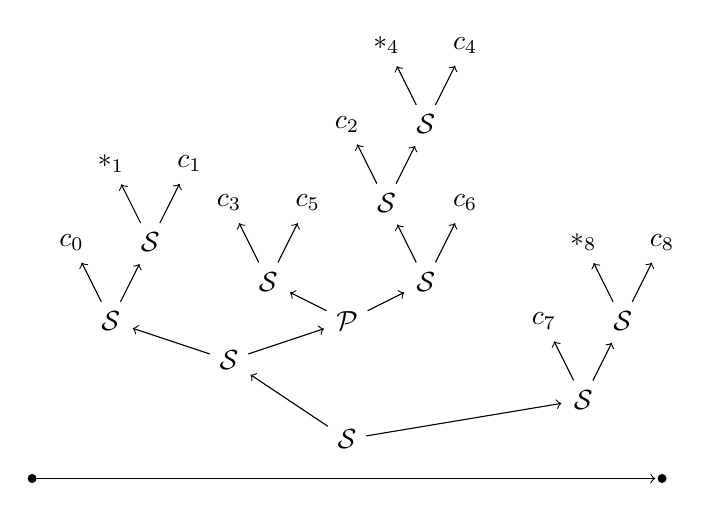
\begin{tikzpicture}[shorten >=1pt, node distance=2cm, on grid, auto]
   \node[circle,draw=black,fill=black,scale=0.3] (c0s) at (0,0) {};
   \node[circle,draw=black,fill=black,scale=0.3] (c8d) at (8,0) {};

   %all
   \node[] (s9) at (2.5,1.5) {$\mathcal{S}$};
   \node[] (s10) at (4,0.5) {$\mathcal{S}$};

   %reduction c0 c1
   \node[] (s1) at (1,2) {$\mathcal{S}$};
   \node[] (c0) at (0.5,3) {$c_0$};
   \node[] (s2) at (1.5,3) {$\mathcal{S}$};
   \node[] (star1) at (1,4) {$*_1$};
   \node[] (c1) at (2,4) {$c_1$};

   %reduction c7 c8
   \node[] (s3) at (7,1) {$\mathcal{S}$};
   \node[] (c7) at (6.5,2) {$c_7$};
   \node[] (s4) at (7.5,2) {$\mathcal{S}$};
   \node[] (star8) at (7,3) {$*_8$};
   \node[] (c8) at (8,3) {$c_8$};

   %reduction c2 c4 c6 c3 c5
   \node[] (p1) at (4,2) {$\mathcal{P}$};
   \node[] (s5) at (3,2.5) {$\mathcal{S}$};
   \node[] (c3) at (2.5,3.5) {$c_3$};
   \node[] (c5) at (3.5,3.5) {$c_5$};
   \node[] (s8) at (5,2.5) {$\mathcal{S}$};
   \node[] (c6) at (5.5,3.5) {$c_6$};
   \node[] (s6) at (4.5,3.5) {$\mathcal{S}$};
   \node[] (c2) at (4,4.5) {$c_2$};
   \node[] (s7) at (5,4.5) {$\mathcal{S}$};
   \node[] (star4) at (4.5,5.5) {$*_4$};
   \node[] (c4) at (5.5,5.5) {$c_4$};
 
  \path[->]
    (c0s) edge node {} (c8d)

    %reduction c0 c1
    (s1) edge node {} (c0)
         edge node {} (s2)
    (s2) edge node {} (star1)
         edge node {} (c1)
    %reduction c7 c8
    (s3) edge node {} (c7)
         edge node {} (s4)
    (s4) edge node {} (star8)
         edge node {} (c8)

    %reduction c2 c4 c6 c3 c5
    (p1) edge node {} (s5)
         edge node {} (s8)
    (s5) edge node {} (c3)
         edge node {} (c5)
    (s8) edge node {} (s6)
         edge node {} (c6)
    (s6) edge node {} (c2)
         edge node {} (s7)
    (s7) edge node {} (star4)
         edge node {} (c4)

    %all
    (s9) edge node {} (s1)
         edge node {} (p1)
    (s10) edge node {} (s9)
          edge node {} (s3);
  \end{tikzpicture}
}
\end{center}
\caption{Big example}
\label{fig:example}
\end{figure}

At this point, the $\mathcal{MSP}$ program can be dumped to any parallel language in which a sequence and a parallel execution are available. For example, we could imagine a parallel functionnal language with a binary \emph{sequence} function and a binary \emph{parallel} function such that the tree of Figure~\ref{fig:t} corresponds the following nested call:

\begin{equation}
\begin{split}
\text{sequence}(a,\text{parallel}(&\\
&\text{sequence}(b,\text{sequence}(\text{parallel}(\text{sequence}(c,d),\text{sequence}(e,f)),g)),\\
&\text{sequence}(h,\text{sequence}(i,j))\\
&))
\end{split}
\end{equation}
%------------------------------------------------------------------------------
% \section{Component-Based Runtime}
% \label{sect:component}
% %----------------------------------------
%\subsection{Overview}
%----------------------------------------
This section describes both the projection of $\Gamma_{tsp}$ to
components, and the remaining needed components to execute a
multi-stencil application. Before those details the section gives an overview of
component models, and introduce the concepts of the Low Level Component Model \llc, which is used in this paper.


%----------------------------------------
\subsection{Component Model Overview}
%----------------------------------------
Component model is a domain of software
engineering~\cite{Szyperski:2002:CSB:515228}, which promotes code
re-use, separations of concerns, and thus maintainability. An
application is made of a set of components; a component being a kind of
black box representing an independent functionnality of the application, and which interacts only through its ports. A port specifies the services provided and required by the component.
%
With respect to high performance computing, some works have also shown
that component models can achieve the needed level of performance, and
scalability while also helping in application
portability~\cite{Bernholdt01052006, bigot:inria-00388508, UCHPC2015}

Many component models exist, each of them with its own specifications
and singularities. In distributed computing, well known component
models are CCM~\cite{corba:omg06} (CORBA Component Model), and
GCM~\cite{Baude} (Grid Component Model); in HPC, there are
CCA~\cite{Bernholdt01052006} (Common Component Architecture), and
\llc~\cite{l2c} (Low Level Component), for example.
%
As this work makes use of \llc, in particular for the experiments, let
introduce concepts of this component model with more details.

%----------------------------------------
\subsection{\llc}
%----------------------------------------

\llc is a minimalist \texttt{C++} based HPC-oriented component model
where a component extends the concept of class by specifying in its
interfaces the services that it offers ($provide$ ports) and that it
needs, either a single service instance ($use$ ports), or multiple
service instances ($use-multiple$ ports). Services are \texttt{C++}
interfaces. \llc also offers $MPI$ ports that enable components to
share MPI communicators. Components can also have attribute ports to
be configured.
%
As illustrated in Figures~\ref{fig:ports}, a $provide$ port is
represented with a white circle, a $use$
port with a black circle, a $use-multiple$ port by a black circle with
a white $m$ in it. MPI port are
connected with a black rectangle.

A classical \llc-based application is a static \emph{assembly} of
components made of instances of components and of connections between
component ports. Such an assembly is described in LAD, an XML
dialect~\cite{l2c}.

\begin{figure}[t]
\begin{center}
\subfloat[][\label{fig:2comp}]{
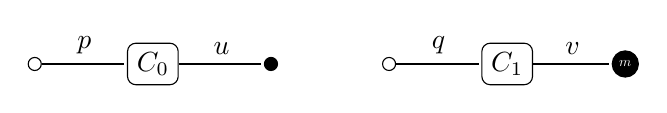
\begin{tikzpicture}[shorten >=1pt, node distance=2cm, on grid, auto]
   \node[component] (C) at (0,0) {$C_0$};
   \node[provide] (p) at (-1.5,0) {};
   \node[use] (u) at (1.5,0) {};
   \node[provide,right=1.5cm of u] (p1) {};
   \node[component,right=1.5cm of p1] (C1) {$C_1$};
   \node[use,right=1.5cm of C1] (um) {$m$};
 
  \path[-]
    (p) edge node {$p$} (C)
    (C.east) edge node {$u$} (u)
    (C1)  edge node {$v$} (um)
    (p1) edge node {$q$} (C1);
\end{tikzpicture}
}
\subfloat[][\label{fig:ass}]{
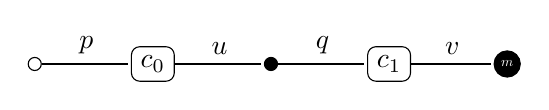
\begin{tikzpicture}[shorten >=1pt, node distance=2cm, on grid, auto]
   \node[component] (C) at (0,0) {$c_0$};
   \node[provide] (p) at (-1.5,0) {};
   \node[use] (u) at (1.5,0) {};
   \node[component,right=1.5 of u] (C1) {$c_1$};
   \node[use,right=1.5 of C1] (um) {$m$};
 
  \path[-]
    (p) edge node {$p$} (C)
    (C) edge node {$u$} (u)
    (C1)  edge node {$v$} (um)
    (u) edge node {$q$} (C1);
\end{tikzpicture}
}
\subfloat[][\label{fig:mpi}]{
\begin{tikzpicture}[shorten >=1pt, node distance=2cm, on grid, auto]
   \node[component] (C) at (0,0) {$c_2$};
   \node[provide] (p) at (-1.5,0) {};
   \node[mpi] (u) at (1.5,0) {};
   \node[component,right=1.5 of u] (C1) {$c_3$};
 
  \path[-]
    (p) edge node {$r$} (C)
    (C) edge node {$m_1$} (u)
    (u) edge node {$m_2$} (C1);
\end{tikzpicture}
}
\caption{Example of components and their ports representation. a) Component $c_0$ has a provide port ($p$) and a use port ($u$); Component $c_1$ has also a provide port ($q$) but also a use multiple port ($v$). b) A use port is connected to a (compatible) provide port. c) Component $c_2$ and $c_3$ shares an MPI communicator.}
\label{fig:ports}
\end{center}
\end{figure}

%% In the rest of this paper, when a required service of a \emph{use} (or \emph{use-multiple}) port is filled and linked to a \emph{provide} port in the comonent assembly, only the use port stay visible, as illustrated in Figure~\ref{fig:assembly}. As the use port is on the right of its component, and the provide port on the left, in a component assembly the component on the left uses the provide port of the component on the right.

%----------------------------------------
\subsection{MSCAC Runtime Overview}
%----------------------------------------

Figure~\ref{fig:mscac:assembly} gives an overview of the back-end component
assembly that is executed. As discusses in Section~\ref{sect:mscac},
there are different types of components. Components~\texttt{Driver},
\texttt{DriverApp}, and \texttt{Time} are always instanciated in the final component assembly; the input MSL file is not used by them except the component \texttt{Time} which uses the terminal \texttt{iteration} of the grammar. There is also a
single Component~\texttt{DDS} (the current version handles a single mesh
type). All these components are provided with the
compiler; dumping this part of the assembly is straightforward.

While Component~\texttt{DDS} is managing the structure of the mesh,
each data of the simulation is handled by a component of type
\texttt{Data}. Therefore, the compiler generates in the assembly as
many instances of such component as needed, from the \texttt{data}
section of an MSL program.

The last part of the assembly is the computation part. Each computation kernel is embedded in a kernel component, denoted K, which have to be written by the user and provided
to the compiler. A kernel component encapsulates a computations. To
access data, a kernel component is connected, by the compiler, to the adequate
\texttt{Data} components such that their ports name respect the names
given in the \texttt{data} section of MSL. We denote the fact that they may have
several use port by adding a star on the use port, as illustrated in Figure~\ref{fig:k}.
\begin{figure}
\begin{center}
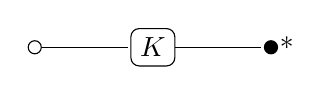
\begin{tikzpicture}[shorten >=1pt, node distance=2cm, on grid, auto]
   \node[component] (k) at (0,0) {$K$};
   \node[provide] (p) at (-1.5,0) {};
   \node[use] (u) at (1.5,0) {};
   \node[right=0.2 of u] (star) {*};
 
  \path[-]
    (p) edge node {} (k)
    (k) edge node {} (u);
\end{tikzpicture}
\end{center}
\caption{Kernel component.}
\label{fig:k}
\end{figure}
  
%% In the computation part of the simulation a final component is needed,
%% the computation component, denoted K. This type of component
%% represents a single computation of the simulation, i.e. the
%% computation of a single output data (written) using a set of input
%% data (read). Using a \emph{use-multiple}, however, a list of component
%% is used and the explicit identification of each component to use is
%% lost. If for SEQ or PAR, the identification of components is not
%% usefull, it is usefull to manipulate data in a computation. For this
%% reason a computation component has as much \emph{use} ports as input
%% and output data to manipulate. We denote this in the bellow
%% representation as a star on the use port.

The rest of the computation part of the assembly contains the static parallel schedule
computed by MSC, \ie $\Gamma_{tsp}$. This is achieved through the use of
three specific components which manage the $P$, $S$, and $sync$
operations of $\Gamma_{tsp}$ as explained hereafter.

%----------------------------------------
\subsection{Control Components}
%----------------------------------------
The series-parallel tree decomposition $\Gamma_{tsp}$ represents the
control of the dependencies of the simulation. As a result to be able
to dump it to a component assembly it is needed to introduce what can
be called \emph{control components}. Those components can be used for
any case of simulation which increases code reuse between
simulations. A control component is composed of a single
\emph{provide} port linked to a single execution method, most of the
time called the \emph{go} method. We introduce three types of control
components represented in Figure~\ref{fig:ctrlcomponents}.

\begin{figure}[t]
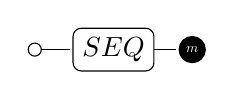
\begin{tikzpicture}[shorten >=1pt, node distance=1cm, on grid, auto]
   \node[component] (seq) at (0,0) {$SEQ$}; \node[provide] (p) at
   (-1,0) {}; \node[use] (u) at (1,0) {$m$};
 
  \path[-]
    (p) edge node {} (seq)
    (seq) edge node {} (u);
\end{tikzpicture}
\hspace{\fill}
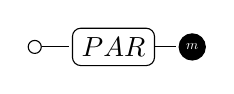
\begin{tikzpicture}[shorten >=1pt, node distance=1cm, on grid, auto]
   \node[component] (seq) at (0,0) {$PAR$};
   \node[provide] (p) at (-1,0) {};
   \node[use] (u) at (1,0) {$m$};
 
  \path[-]
    (p) edge node {} (seq)
    (seq) edge node {} (u);
\end{tikzpicture}
\hspace{\fill}
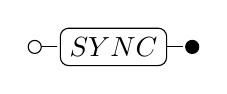
\begin{tikzpicture}[shorten >=1pt, node distance=1cm, on grid, auto]
   \node[component] (sync) at (0,0) {$SYNC$};
   \node[provide] (p) at (-1,0) {};
   \node[use] (u) at (1,0) {};
 
  \path[-]
    (p) edge node {} (sync)
    (sync) edge node {} (u);
\end{tikzpicture}
\\
a) Comp. SEQ
\hspace{\fill}
b) Comp. PAR
\hspace{\fill}
c) Comp. SYNC
\\
\caption{The three control components used by the back-end.}
\label{fig:ctrlcomponents}
\end{figure}

\begin{description}
\item[Sequence component (SEQ)] It is the direct representation of a sequence node of $\Gamma_{tsp}$. The role of this component is to call an ordered list of other components. Its interface contains an ordered \emph{use-multiple} port to be connected to the components to call in sequence.

\item[Parallel component (PAR)] It is the direct representation of a parallel node of $\Gamma_{tsp}$. The role of this component is to call simultaneously a set of other components. It offers a \emph{use-multiple} port to be connected to the components to call in parallel.
  
\item[Synchronization component (SYNC)]. It is the direct representation to an update leaf of $\Gamma_{tsp}$. The role of this component is to call the synchronization of a given data. It offers a \emph{use} port to be connected to the data to update.

\end{description}


%----------------------------------------
\subsection{Dump To Component Assembly}
%----------------------------------------
From $\Gamma_{tsp}$ and using the control components described above,
a direct dump can be done to a component assembly for an hybrid (data
and task) parallelization of a simulation. 
\fix{HC: ce qui suit est a changer avec la fusion du code de plusieurs composants}
However, it is also
possible to dump to a data parallelization only. In such a case the
computation of $\Gamma_{sync}$ is enough to generate the component
assembly. Actually a single SEQ component is thus needed and this
component is linked to all computations and synchronizations of
$\Gamma_{sync}$ directly.

Figure~\ref{fig:tsp:assembly} displays the assembly part corresponding to
$\Gamma_{tsp}$ of Figure~\ref{fig:tsp}. In this figure, the ports
linked to data (use and use-multiple ports of SYNC and K) are
represented but are not connected. Moreover, each computation
component is an instance of the component K presented before but using
the identification name of the computation in the MSL file.

\begin{figure*}[t]
\begin{center}
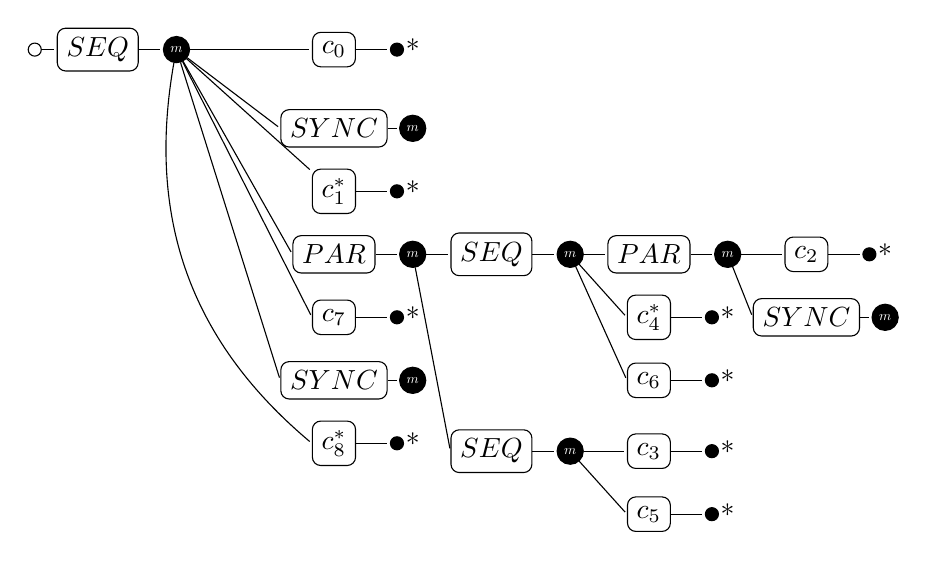
\begin{tikzpicture}[shorten >=1pt, node distance=2cm, on grid, auto]
   %seq0
   \node[component] (seq0) at (0,0) {$SEQ$};
   \node[provide] (seq0p) [left = 0.8cm of seq0] {};
   \node[use] (seq0u) [right = 1cm of seq0] {$m$};
   %c0
   \node[component] (c0) [right = 2cm of seq0u] {$c_0$};
   \node[use] (c0u) [right = 0.8cm of c0] {};
   \node[right=0.2 of c0u] (star) {*};
   %sync0
   \node[component] (sync0) [below = 1cm of c0] {$SYNC$};
   \node[use] (sync0u) [right = 1cm of sync0] {$m$};
   %c1
   \node[component] (c1) [below = 0.8cm of sync0] {$c_1^*$};
   \node[use] (c1u) [right = 0.8cm of c1] {};
   \node[right=0.2 of c1u] (star) {*};
   %par0
   \node[component] (par0) [below = 0.8cm of c1] {$PAR$};
   \node[use] (par0u) [right = 1cm of par0] {$m$};
  %seq1
   \node[component] (seq1) [right = 1cm of par0u] {$SEQ$};
   \node[use] (seq1u) [right = 1cm of seq1] {$m$};
   %par1
   \node[component] (par1) [right = 1cm of seq1u] {$PAR$};
   \node[use] (par1u) [right = 1cm of par1] {$m$};
  %c2
   \node[component] (c2) [right = 1cm of par1u] {$c_2$};
   \node[use] (c2u) [right = 0.8cm of c2] {};
   \node[right=0.2 of c2u] (star) {*};
  %sync1
   \node[component] (sync1) [below = 0.8cm of c2] {$SYNC$};
   \node[use] (sync1u) [right = 1cm of sync1] {$m$};
  %c4
   \node[component] (c4) [below = 0.8cm of par1] {$c_4^*$};
   \node[use] (c4u) [right = 0.8cm of c4] {};
   \node[right=0.2 of c4u] (star) {*};
  %c6
   \node[component] (c6) [below = 0.8cm of c4] {$c_6$};
   \node[use] (c6u) [right = 0.8cm of c6] {};
   \node[right=0.2 of c6u] (star) {*};
  %seq2
   \node[component] (seq2) [below = 2.5cm of seq1] {$SEQ$};
   \node[use] (seq2u) [right = 1cm of seq2] {$m$};
  %c3
   \node[component] (c3) [right = 1cm of seq2u] {$c_3$};
   \node[use] (c3u) [right = 0.8cm of c3] {};
   \node[right=0.2 of c3u] (star) {*};
  %c5
   \node[component] (c5) [below = 0.8cm of c3] {$c_5$};
   \node[use] (c5u) [right = 0.8cm of c5] {};
   \node[right=0.2 of c5u] (star) {*};
  %c7
   \node[component] (c7) [below = 0.8cm of par0] {$c_7$};
   \node[use] (c7u) [right = 0.8cm of c7] {};
   \node[right=0.2 of c7u] (star) {*};
  %sync2
   \node[component] (sync2) [below = 0.8cm of c7] {$SYNC$};
   \node[use] (sync2u) [right = 1cm of sync2] {$m$};
  %c8
   \node[component] (c8) [below = 0.8cm of sync2] {$c_8^*$};
   \node[use] (c8u) [right = 0.8cm of c8] {};
   \node[right=0.2 of c8u] (star) {*};

   \path[-]
   %seq0
    (seq0) edge node {} (seq0u)
    (seq0p) edge node {} (seq0)
   %c0
    (seq0u) edge node {} (c0)
    (c0) edge node {} (c0u)
    %sync0
    (seq0u) edge node {} (sync0.west)
    (sync0) edge node {} (sync0u)
    %c1
    (seq0u) edge node {} (c1)
    (c1) edge node {} (c1u)
   %par0
    (seq0u) edge node {} (par0.west)
    (par0) edge node {} (par0u)
  %seq1
    (par0u) edge node {} (seq1)
    (seq1) edge node {} (seq1u)
  %par1
    (seq1u) edge node {} (par1.west)
    (par1) edge node {} (par1u)
  %c2
    (par1u) edge node {} (c2)
    (c2) edge node {} (c2u)
  %sync0
    (par1u) edge node {} (sync1.west)
    (sync1) edge node {} (sync1u)
  %c4
    (seq1u) edge node {} (c4.west)
    (c4) edge node {} (c4u)
  %c6
    (seq1u) edge node {} (c6.west)
    (c6) edge node {} (c6u)
  %seq2
    (par0u) edge node {} (seq2.west)
    (seq2) edge node {} (seq2u)
  %c3
    (seq2u) edge node {} (c3)
    (c3) edge node {} (c3u)
  %c6
    (seq2u) edge node {} (c5.west)
    (c5) edge node {} (c5u)
  %c6
    (seq0u) edge node {} (c7.west)
    (c7) edge node {} (c7u)
  %sync2
    (seq0u) edge node {} (sync2.west)
    (sync2) edge node {} (sync2u)
  %c8
    (seq0u) edge [bend right] node {} (c8.west)
    (c8) edge node {} (c8u)
   ;
\end{tikzpicture}
\caption{Component assembly representing the computation part generated from $\Gamma_{tsp}$ of Figure~\ref{fig:tsp}.}
\label{fig:tsp:assembly}
\end{center}
\end{figure*}

%----------------------------------------

%------------------------------------------------------------------------------
% \section{Evaluation}
% \label{sect:eval}
% This section evaluates the MSL compiler and the code it generates.
We first evaluate the generated code in the case where only data parallelization and fusion are applied and compare this to a full SkelGIS program.
Then, we analyze a case taking advantage of the full the hybrid parallelization combining data and task parallelism and validate the performance model proposed in Section~\ref{sect:tsp}.

All evaluations presented in this section are based on a real case study of the shallow-Water Equations as solved in  the FullSWOF2D\footnote{\url{http://www.univ-orleans.fr/mapmo/soft/FullSWOF/}}~\cite{Ferrari2004,CPE:CPE3494} code from the MAPMO laboratory, University of Orl\'eans.
We have developed a MSL version of FullSWOF2D that contains 3~mesh entities, 7~computation domains, 48~data and 98~computations (32~stencil kernels and 66~local kernels).

%-------------------------------------
\subsection{Compiler}

Table~\ref{fig:exectime} illustrates the execution time for each step of the MSL compiler for the FullSWOF2D example.
This has been computed on a laptop with a bi-core Intel Core i5 1.4~GHz, and 8~GB of DDR3.
While the overall time of 4.6 seconds remains reasonable, one can notice that the computation of the $TSP$ tree is by far the longest step of the compiler.
As a matter of fact, the complexity of the algorithm for N-shapes removal is $O(n^3)$.
The replacement of the static scheduling by a direct scheduling of the DAG by dedicated tools should solve this in the future.

\begin{table}[!h]
 \begin{center}
 \begin{tabular}{|c|c|c|c|c|}
  \hline
   Step & Parser & $\Gamma_{sync}$ & $\Gamma_{dep}$ & $TSP$\\
   \hline
   Time (ms) & 1 & 2 & 4.2 & 3998.5\\
   \hline
   \% & 0.022 & 0.043 & 0.09 & 86.6\\
   \hline
 \end{tabular}
\caption{Execution times of the MSL compiler}
\label{fig:exectime}
 \end{center}
\end{table}

%-------------------------------------
\subsection{Data parallelism}

The first parallelization technique proposed by MSL is a data parallelization. To implement this parallelization, the dump step of the MSL compiler uses the SkelGIS language. This language, as already described, offers a distributed Cartesian mesh and programming interfaces to use it as a sequential data structure. It has been evaluated itself compared to an MPI implementation on the same FullSWOF2D simulation~\cite{CPE:CPE3494}. What MSL brings to SkelGIS is an automatic detection of where MPI synchronizations are needed during the numerical simulation, and how to make a fusion of some computations in order to reduce cache misses. This section gives a performance comparison of the code produced by MSL for FullSWOF2D, and of the equivalent manual SkelGIS program (with manual synchronizations and fusion choices). Moreover, as the code produced by MSL is a component-based code, this evaluation also shows that no overheads are introduced \llc~\cite{l2c}. Following evaluations have been performed onto the machine of the TGCC Curie described in Table~\ref{tab:TGCC}. Each evaluation has been performed ten times and the median is presented in results.

\begin{table}[!h]
\begin{center}
 \begin{tabular}{|c|c|}
   \hline
    Cluster & \textbf{TGCC Curie Thin Nodes}\\
     \hline         
    Processor & 2$\times$SandyBridge\\
    & (2.7 GHz)\\
    Cores/node & 16 \\
    RAM/node & 64 GB\\
    RAM/core & 4GB\\
    Compiler [-O3] & gcc 4.9.1\\
    MPI & Bullxmpi\\
    Network & Infiniband\\
    \hline
 \end{tabular}
 \caption{\label{tab:TGCC}Hardware configuration of TGCC Curie Thin nodes.}
 \end{center}
\end{table}

\paragraph{\textbf{Weak scaling}} The first evaluation is a weak scaling evaluation. In a weak scaling, a constant amount of work is given to each core while increasing the overall number of cores. As a result, the overall domain size also increase with the number of cores. A weak scaling is a good evaluation to detect overheads which are independent from the amount of computation performed by each core, such as collective communications, or overheads introduced by \llc components, for example. Figures~\ref{fig:weak1} and~\ref{fig:weak2} respectively show the weak scaling evaluations for a $400 \times 400$ and a $800 \times 800$ domain for each core, from 16 cores to 16.384 cores. Minimum and maximum values are also shown as error bars in figures.

\begin{figure}[!h]\begin{center}
  \resizebox{8cm}{!}{\includegraphics{../results/weak_scaling/400/median_weak.pdf}}
  \caption{weak-scaling with $400 \times 400$ domain per core.}
  \label{fig:weak1}
\end{center}\end{figure}
\begin{figure}[!h]\begin{center}
  \resizebox{8cm}{!}{\includegraphics{../results/weak_scaling/800/median_weak.pdf}}
  \caption{weak-scaling with $800 \times 800$ domain per core.}
  \label{fig:weak2}
\end{center}\end{figure}

One can notice that the MSL code produces a better execution time on the $400 \times 400$ domain, while it produces a small overhead on the $800 \times 800$ domain. Those results could be due to different optimizations of the gcc compiler due to components. Actually, a component in \llc is compiled independently, as an dynamic library, with the \emph{-fpic} compilation option, while the SkelGIS version is compiled entirely as a single code. However, one can also notice that except those not significant differences of execution times, weak scalings have the same behavior on both codes.

\paragraph{\textbf{Strong scaling}} The second evaluation is a strong scaling evaluation. Unlike a weak scaling, a strong scaling keeps a constant overall size of problem, while the number of cores increase. As a result, the sub-domain computed by each core reduces while the number of cores increases. The strong scaling is a good additional evaluation to the weak scaling, showing different kinds of overheads, such as cache misses (when the size of sub-domain becomes small enough to fit into cache memory), or small constant overheads. Figure~\ref{fig:strong} shows the strong scaling evaluation for a $10k \times 10k$ overall domain size, from 16 cores to 16.384 cores. This strong scaling is illustrated with the number of iterations per seconds as a function of the number of cores. The ideal strong scaling is also illustrated.

\begin{figure}[!h]\begin{center}
  \resizebox{8cm}{!}{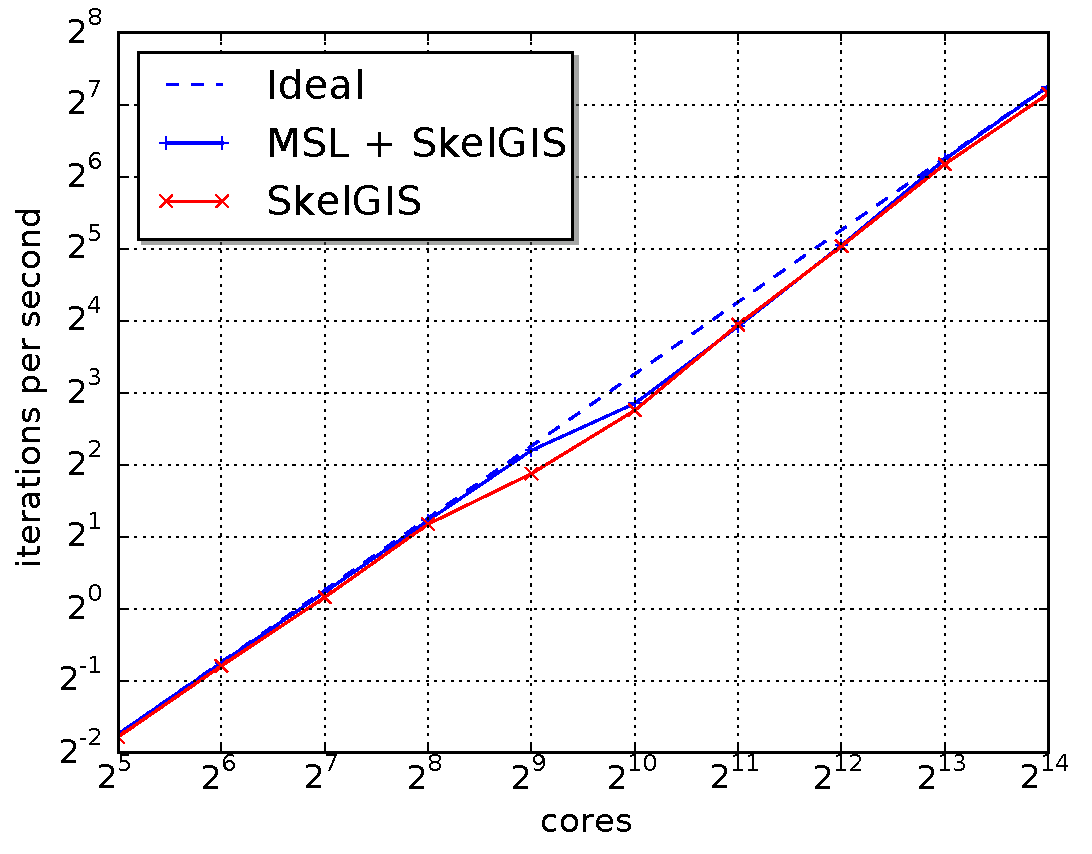
\includegraphics{../results/strong_scaling/10K_1K/median_strong.pdf}}
  \caption{Strong scaling on a $10k \times 10k$ domain.}
  \label{fig:strong}
\end{center}\end{figure}

First, one can notice that the strong scaling evaluated for the code generated by MSL is close to the ideal speedup up to 16.384 cores, which is a very good result. Moreover, no overheads are introduced by MSL which shows that automatic synchronization detections and automatic fusion detections are the same one that the one written manually into the SkelGIS code of FullSWOF2D. Finally, no overheads are introduced by components of \llc. A small behavior difference can be noticed with $2^9=512$ cores, however this variation is no longer observed with 1024 cores.

\paragraph{\textbf{Fusion}} Finally, to evaluate the data parallelization technique automatically introduced by MSL, the fusion optimization is evaluated. Figure~\ref{fig:fusion} shows the number of iterations per second as a function of the number of cores, for FullSWOF2D with and without fusion optimization and onto a $500 \time 500$ domain. As explained in Section~\ref{sect:fusion}, the MSL fusion happens at a high level and is most of the time done naturally by a computer scientist. However, for a non computer scientist which write its numerical codes, an automatic proposition of such fusions makes the implementation easier. Moreover, one can notice that the performance is clearly improved (around 40\%) by this fusion.

\begin{figure}[!h]\begin{center}
  \resizebox{8cm}{!}{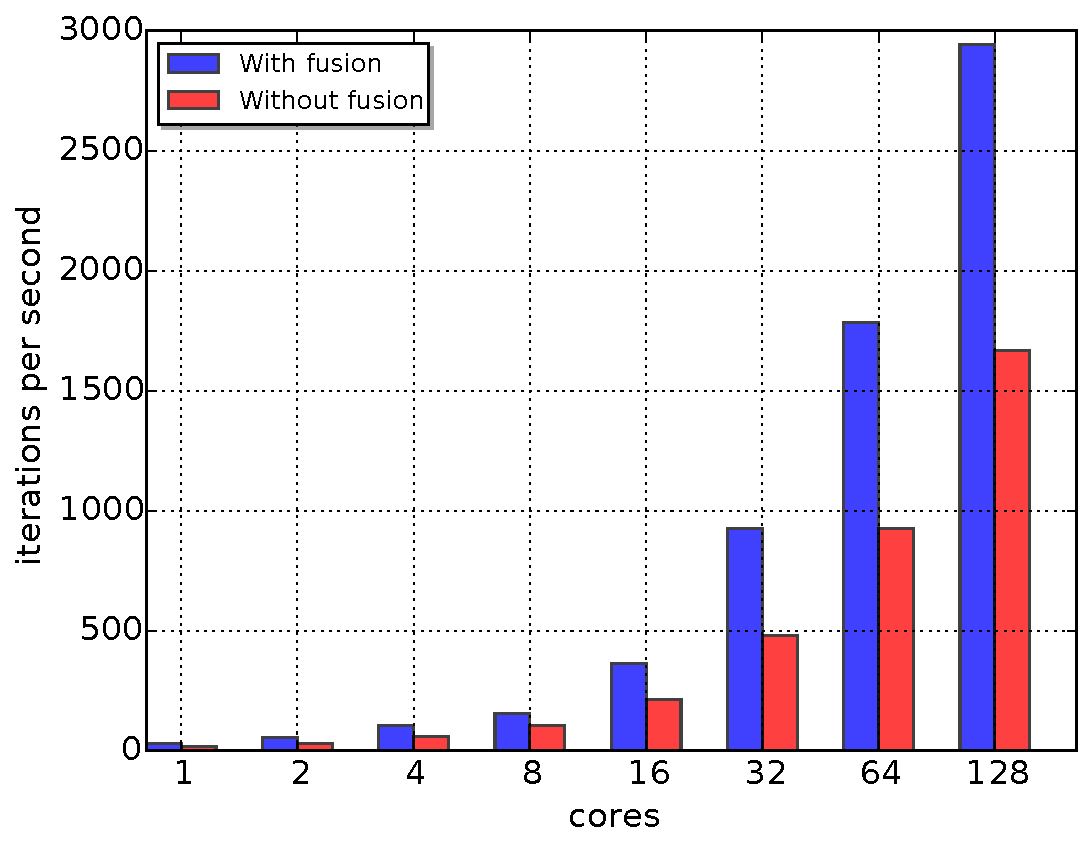
\includegraphics{../results/task_scaling/500_200/fusVSbase.pdf}}
  \caption{Strong scaling on a 500x500 domain, with and without the fusion optimization.}
  \label{fig:fusion}
\end{center}\end{figure}

%-------------------------------------
\subsection{Hybrid parallelism}

The series-parallel tree decomposition $TSP$ of this simulation, extracted by the MSL compiler, is composed of 17~sequence nodes and 18~parallel nodes. Table~\ref{fig:freq} represents the number of time a given level of parallelism, \ie the number of tasks to perform concurrently, is observed in the final tree. One can notice that the level of task parallelism extracted from the Shallow water equations is limited by two sequential parts in the application (level 1). Moreover, a level of 16~parallel tasks is reached two times, and five times for the fourth level.
This means that if two threads are dedicated to task parallelism, two parts of the code at least will not take advantage of this and that no part of the code would benefit from more than 16 threads.

\begin{table}[!h]
 \begin{center}
 \begin{tabular}{|c|c|c|c|c|c|c|c|c|}
    \hline 
   Level & 1 & 2 & 3 & 4 & 6 & 10 & 12 & 16\\
   \hline
   Frequency & 2 & 1 & 3 & 5 & 3 & 1 & 1 & 2\\
   \hline
 \end{tabular}
\caption{Parallelism level (number of parallel tasks) and the number of times this level appears.}
\label{fig:freq}
 \end{center}
\end{table}

The second parallelization technique proposed by MSL is an hybrid parallelization which mixes data parallelization and task parallelization. To implement this hybrid parallelization, the dump step of the MSL compiler uses the SkelGIS language, and the OpenMP language.

First, Figure~\ref{fig:limit} illustrates limitations of data parallelization technique alone. As explained in Section~\ref{sect:perfs}, performance of data parallelism is limited by the communication time between resources. As a result, when the size of sub-domain for each core becomes too small, and as the communication time increases with the number of cores, the strong speedup of the data parallelization starts to bend down. To catch this phenomena without too much cores, a relatively small domain of $500 \times 500$ is used.

\begin{figure}[!h]\begin{center}
  \resizebox{8cm}{!}{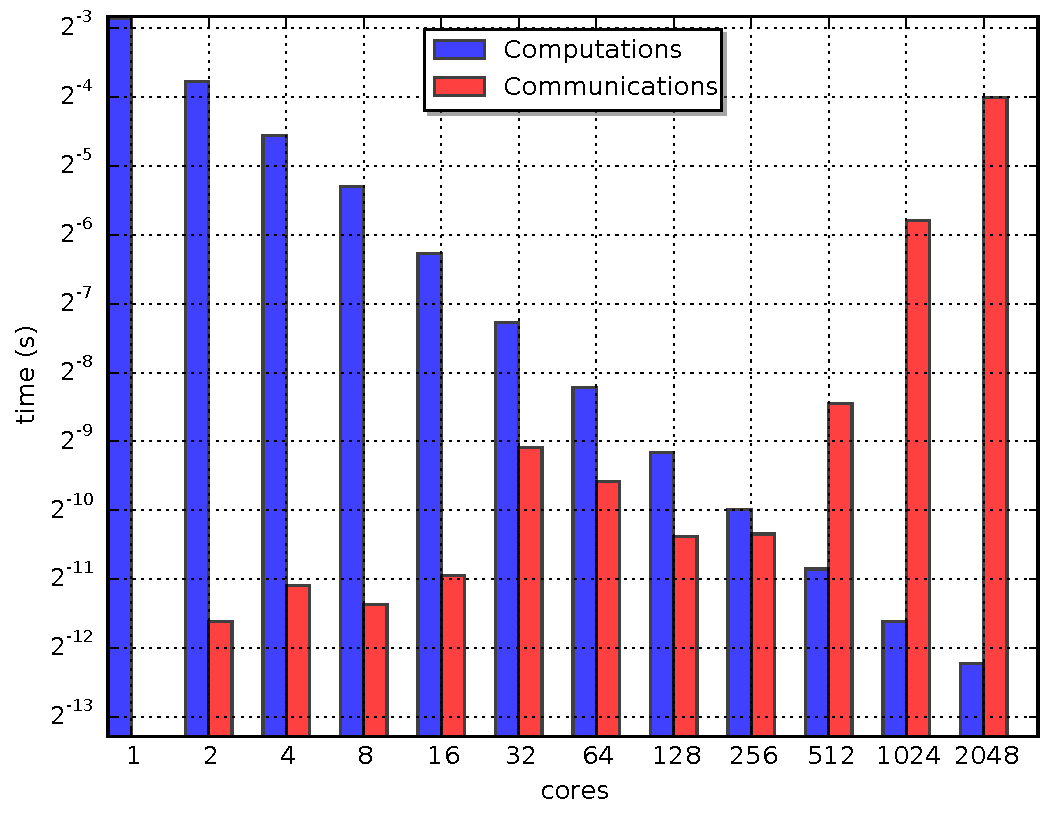
\includegraphics{../results/task_scaling/500_200/analytic/times.pdf}}
  \caption{Computation vs communication times in the data parallelization technique.}
  \label{fig:limit}
\end{center}\end{figure}

As expected, from 1 to 2048 cores the computation times decrease linearly. On the other hand, from 1 to 256 cores the communication time is almost constant, but from 256 to 2048 cores it increases. As a result from 512 cores to 2048 cores, the communication time becomes greater than the computation time. In Figure~\ref{fig:close}, the blue curve shows the strong scaling of the same example. Thus, from 256 to 2048 cores, the speedup bends down.

\medskip
In addition to the blue curve, Figure~\ref{fig:close} shows strong scalings for the same example but using an hybrid parallelization. For example, the purple curve shows the parallelization which uses 8 cores, to perform the task parallelization, for each process used for data parallelization (\ie MPI process). As a result, for example, when using 2 machines of the TGCC cluster, with a total of 32 cores, 4 cores are used for SkelGIS MPI processes, for data parallelization, and for each one 8 cores are used for task parallelization ($4 \times 8 = 32$).

As a result, and as explained in Section~\ref{sect:perfs}, data is less divided into sub-domains and the effect which is observe onto the blue curve is delayed. This figure shows a comparison with 2, 4, 8 and 16 cores per MPI process for task parallelization.

\begin{figure}[!h]\begin{center}
  \resizebox{8cm}{!}{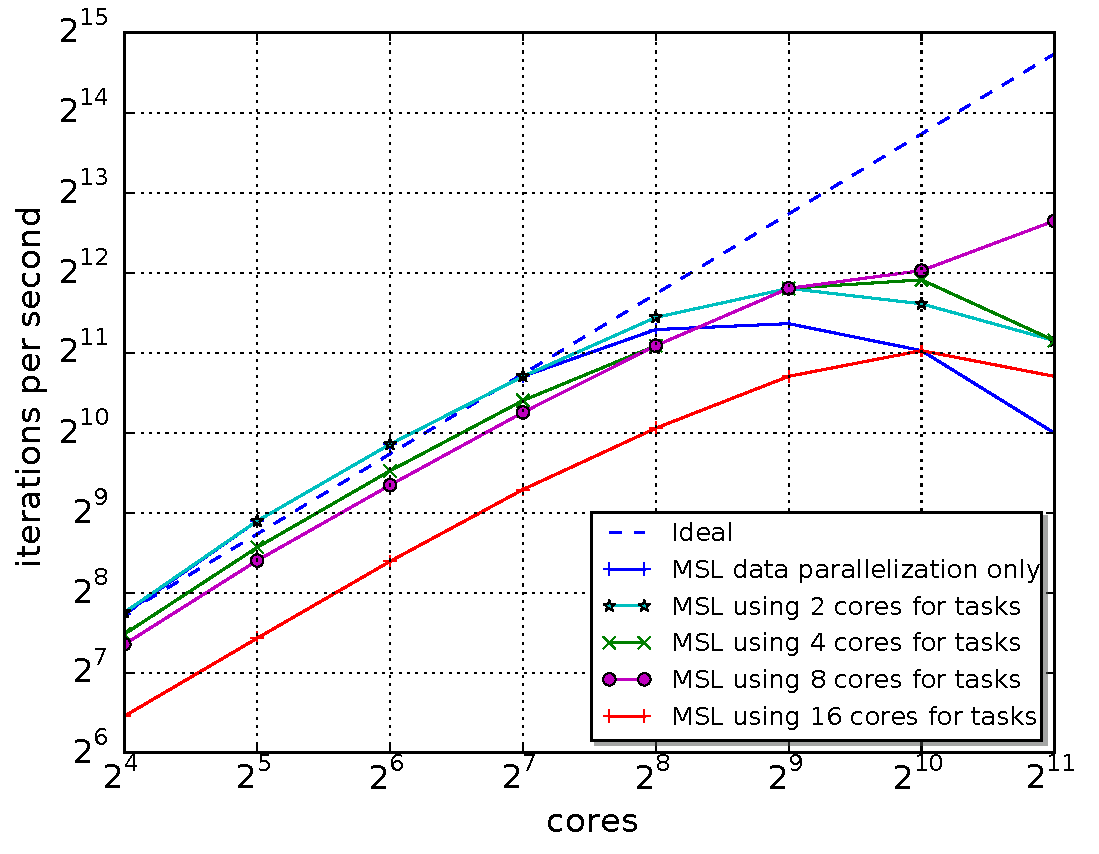
\includegraphics{../results/task_scaling/500_200/base_close_median.pdf}}
  \caption{Strong scaling comparisons between data parallelization and hybrid parallelization. A \emph{close} OpenMP clause is used to bind threads onto cores.}
  \label{fig:close}
\end{center}\end{figure}

From 2 to 8 cores, the improvement of the strong scaling is clear. However, reaching 16 cores, an important initial overhead appears and in addition to this, the curve bends down rapidly instead of improving the one with 8 cores for task parallelization. Two different phenomena happen.

First, thin nodes of the TGCC Curie are built with two NUMA nodes each of 8 cores. As a result, when increasing the number of OpenMP cores for task parallelization from 8 to 16 cores, an overhead is introduced by exchanges of data between memories of the two NUMA nodes. This phenomena is illutrated in Figure~\ref{fig:spread}. In this figure, a different strategy is used to bind threads onto available cores (using OpenMP). This strategy, called \emph{spread} instead of \emph{close} in Figure~\ref{fig:close}, binds threads on cores in order to spread as much as possible onto resources, which means that the two NUMA nodes are directly used whatever the number of cores kept for task parallelization. As a result, and as shown in the figure, using 2, 4 and 8 cores an initial overhead is introduced.

\begin{figure}[!h]\begin{center}
  \resizebox{8cm}{!}{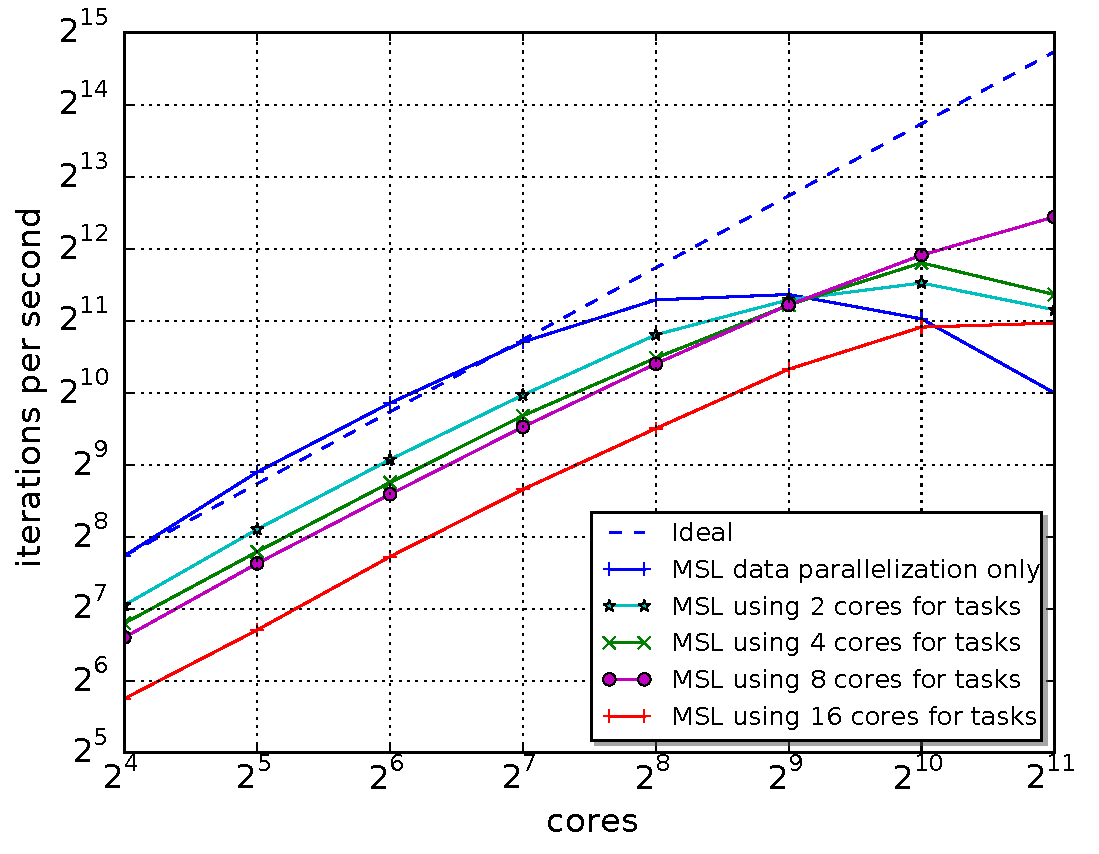
\includegraphics{../results/task_scaling/500_200/base_spread_median.pdf}}
  \caption{Strong scaling comparisons between data parallelization and hybrid parallelization. A \emph{spread} OpenMP clause is used to bind threads onto cores.}
  \label{fig:spread}
\end{center}\end{figure}

The second phenomena, which happens in Figure~\ref{fig:close} with 16 cores for tasks parallelization, is due to the level of parallelization introduced by the task parallelization technique. Actually, as illustrated in Table~\ref{fig:freq}, only two steps of the $TSP$ static scheduling generated by the MSL compiler can take advantage of 16 cores among a total of 18 steps. This phenomena has been explained in Section~\ref{sect:perfs} by the variable $F_{task}$ and the fact that it is not always true that $F_{task}=P_{task}$. This explains why using 16 cores for task parallelization in Figure~\ref{fig:spread} is still less efficient than using 8 cores even if the two NUMA nodes are always used in this evaluation.

Finally, to completely validate the performance model introduced in Section~\ref{sect:perfs}, and to understand when the hybrid parallelization becomes more interesting than the data parallelization, Figure~\ref{fig:tth2} represents $T_{COM1}$ and $T_{COM2}+T_{task}$ of Equation~(\ref{eq:hyb}), for the best case, \ie when 8 cores are used for task parallelization, and with a \emph{close} OpenMP bind of threads onto cores. Table~\ref{fig:tth} gives time details.

\begin{table}[!h]
 \begin{center}
 \begin{tabular}{|c|c|c|c|c|}
    \hline 
    & $T_{COM1}$ & $T_{COM2}$ & $T_{task}$ & Equation~(\ref{eq:hyb})\\
   \hline
   16 cores ($2 \times 8$) & 0.0005 & 0.00032 & 0.013 & False\\
   32 cores ($4 \times 8$) & 0.0018 & 0.00045 & 0.0062 & False\\
   64 cores ($8 \times 8$) & 0.0013 & 0.00038 & 0.0034 & False\\
   128 cores ($16 \times 8$) & 0.00075 & 0.0005 & 0.0023 & False\\
   256 cores ($32 \times 8$) & 0.00077 & 0.0018 & 0.001 & False\\
   512 cores ($64 \times 8$) & 0.0029 & 0.0013 & 0.00052 & True\\
   1024 cores ($128 \times 8$) & 0.018 & 0.00075 & 0.00029 & True\\
   2048 cores ($256 \times 8$) & 0.0623 & 0.00077 & 0.00016 & True\\
   \hline
 \end{tabular}
\caption{Execution times (seconds) of $T_{COM1}$, $T_{COM2}$ and $T_{task}$ for 8 cores for task parallelization. Verification of the Equation~(\ref{eq:hyb}).}
\label{fig:tth}
 \end{center}
\end{table}

\begin{figure}[!h]\begin{center}
  \resizebox{8cm}{!}{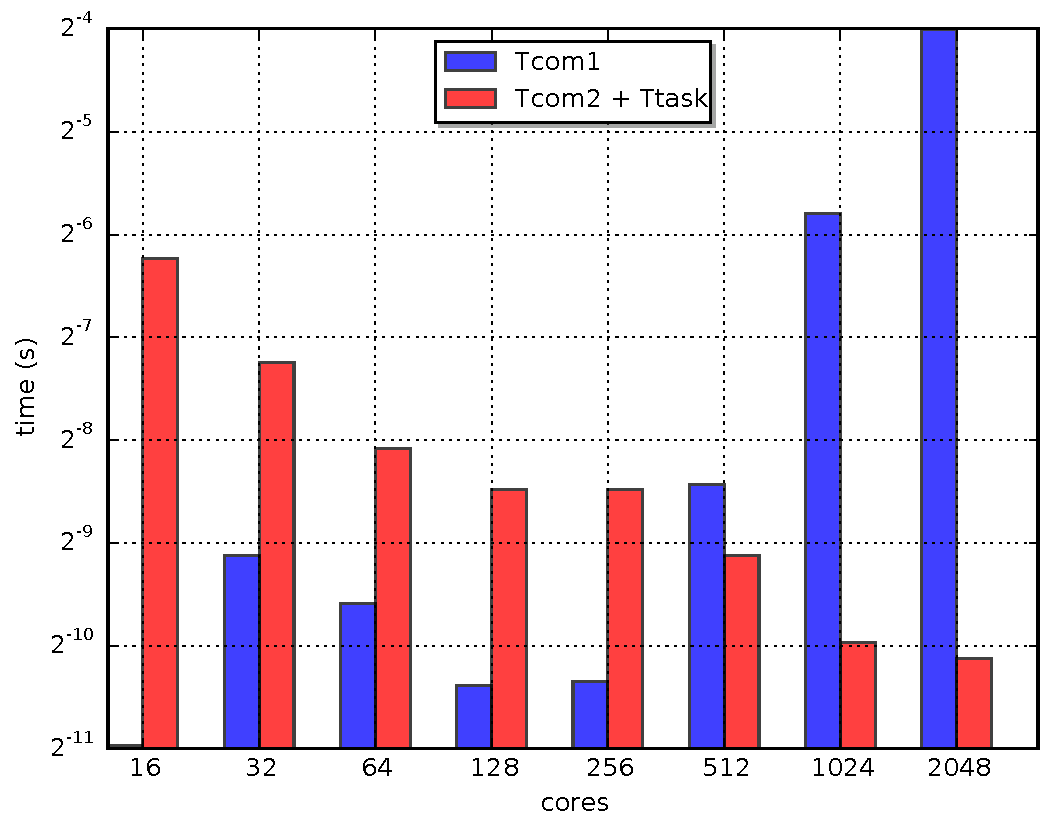
\includegraphics{../results/task_scaling/500_200/analytic/tth.pdf}}
  \caption{Execution times (seconds) of $T_{COM1}$ and $T_{COM2} + T_{task}$ for 8 cores for task parallelization. Verification of the Equation~(\ref{eq:hyb}).}
  \label{fig:tth2}
\end{center}\end{figure}

Figure~\ref{fig:tth2} and Table~\ref{fig:tth} perfectly matches results observed in Figure~\ref{fig:close} for 8 cores used for task parallelization per core used for data parallelization. As a result, the hybrid parallelization becomes better with a total of 512 cores.

%------------------------------------------------------------------------------
% \section{Related work}
% \label{sect:rel}
% stencil compilation: Pochoir, PATUS etc.\\
stencil programs: Lizst, OP2\\
control in components: X-MAN (The New Component Model), STCM, Kell-calculus
%------------------------------------------------------------------------------
% \section{Conclusion}
% \label{sect:concl}
% This paper has presented the domain specific language MSL and its compiler MSCAC designed to produce a parallel (data and hybrid) component-based runtime of an overall multi-stencil program, \ie a mesh-based numerical simulation reduced to explicit schemes. After details on the language and its compiler, MSL has been evaluated by the description of a real case numerical simulation: the shallow water equations. The component-based data parallelization of the simulation has been compared to a pure SkelGIS parallelization, and has shown improved execution times as well as a promising scalability. Those results demonstrate that component-based runtimes may be relevant back-end codes for DSLs as they do not introduce performance damage. Moreover, components bring software engineering benefits such as separation of concerns, code re-use, improving maintainability.

Although MSL is a promising case study from DSLs to component-based runtimes, many works in progress aims at improving this first contribution. First, to more clearly show the improvement of DSLs maintainability using component-based back-end, an alternative \texttt{DDS} component is under study, using Global Arrays~\cite{Nieplocha:2006:AAP:1125980.1125985}. In addition to this, alternatives for the \texttt{Computations} component, computed by MSC, are under study such as a dump to a pure OpenMP~\cite{660313} code or the use of dynamic schedulers~\cite{Augonnet2011,Gautier:2013:XRS:2510661.2511383}. %This last work on dynamic schedulers could also improve the expressivity of task parallelism in MSL, as discussed in Section~\ref{sect:eval}. Thus, it could bring interesting performance for the hybrid parallelization.

%------------------------------------------------------------------------------
\label{sect:bib}
\bibliographystyle{plain}
\bibliography{biblio}

\end{document}
\endinput
%%
%% End of file `squelette-rr.tex'.
